\documentclass[12pt]{report}
\usepackage{graphicx}
\usepackage{array}
\usepackage{tabularx}
\usepackage{amsmath}
\usepackage{hyperref}
\usepackage{geometry}
\usepackage{fontspec} % For custom fonts
\usepackage{xcolor}
\usepackage{float}
\usepackage{titling}
\usepackage{tikz}
\usepackage{longtable}
\usepackage{fancyhdr} % For custom headers/footers
\usepackage{tocbibind} % To include TOC, LOF, LOT in TOC
\setmainfont{Times New Roman} % Set the main font to Times New Roman
\geometry{a4paper, margin=1in}
\usepackage{setspace}
\onehalfspacing 
\usepackage{titlesec}
\usepackage{fancyhdr}
\usepackage[titles]{tocloft}
\usepackage{chngcntr}

\counterwithout{figure}{chapter}
\counterwithout{table}{chapter}

\renewcommand{\tablename}{Tableau}
\renewcommand{\cftpartpresnum}{PARTIE~} 
\renewcommand{\cftpartaftersnum}{.}     
\renewcommand{\cftpartleader}{\cftdotfill{\cftdotsep}}
\setlength{\cftpartnumwidth}{5em}

\renewcommand{\cftchappresnum}{Chapitre~}
\renewcommand{\cftchapaftersnum}{.}     
\renewcommand{\cftchapleader}{\cftdotfill{\cftdotsep}}
\setlength{\cftchapnumwidth}{5em}

\pagestyle{fancy}
\fancyhf{} % Clear all header and footer fields
\fancyfoot[C]{\thepage} % Place the page number in the center of the footer
\renewcommand{\headrulewidth}{0pt}  % Removes the line in the header
\renewcommand{\footrulewidth}{0pt}  % Removes the line in the footer
\hypersetup{
   colorlinks=true,
  linkcolor=black,   % Set link color to black
  filecolor=magenta, 
  urlcolor=cyan,
  pdfborder={0 0 0} 
}
\renewcommand{\contentsname}{SOMMAIRE GENERAL} 
\renewcommand{\listtablename}{LISTE DES TABLEAUX}
\renewcommand{\listfigurename}{LISTE DES FIGURES}
\newcommand{\figref}[1]{figure \ref{#1}}

\titleformat{\part}[display]
  {\normalfont\Huge\bfseries\centering}
  {PARTIE \Roman{part}}{20pt}{\Huge}

\titleformat{\chapter}[display]
  {\normalfont\Large\bfseries\centering}
  {Chapitre \arabic{chapter}~.}{20pt}{\Large}

\titleformat{\section}
    {\normalfont\large\bfseries} 
    {\thesection}
    {1em}
    {\large}

\titleformat{\subsubsection}
    {\normalfont\Large\bfseries} 
    {\thesubsubsection}
    {1em}
    {\large}
	
\setcounter{secnumdepth}{5}
\renewcommand{\thesubsubsection}{\alph{subsubsection}}
\makeatletter \renewcommand\paragraph{\@startsection{paragraph}{4}{\z@}{3.25ex \@plus1ex \@minus.2ex}{1ex \@plus.2ex}{\normalfont\normalsize\bfseries}} \renewcommand\theparagraph{$\bullet$}
\renewcommand\subparagraph{\@startsection{subparagraph}{5}{\z@}{3.25ex \@plus1ex \@minus.2ex}{1ex \@plus.2ex}{\normalfont\normalsize\bfseries}} \renewcommand\thesubparagraph{$-$} \makeatother
\begin{document}	
			 \pretitle{
				\begin{tikzpicture}[remember picture, overlay]
			   		\node[anchor=north west, xshift=1.5cm, yshift=-1cm] at (current page.north west) {
        						\includegraphics[width=2.5cm]{image1.png}
					};
    					\node[anchor=north west, xshift=4cm, yshift=-1cm] at (current page.north west) {
        						\includegraphics[width=2.3cm]{image2.png}
					};
					\node[anchor=north east, xshift=-1.5cm, yshift=-1cm] at (current page.north east) {
        						
\includegraphics[width=5cm]{image3.png}
					};
				\end{tikzpicture}
				\begin{center}
					\textbf{\large UNIVERSITE DE FIANARANTSOA ECOLE NATIONALE D'INFORMATIQUE \\[0.5cm] MEMOIRE DE FIN D'ETUDES POUR L'OBTENTION DU DIPLOME DE MASTER PROFESSIONNELLE}
					\\[0.5cm]
							\textbf{\underline{Mention:}} Informatique \\	
							\textbf{\underline{Parcours:}} Informatique générale\\
							\textbf{\textit{Intitulé}}				\end{center}
				\begin{center}\Large\bfseries
			}
			\preauthor{\begin{flushleft}\fontsize{12} \lineskip Présenté le 01 février 2023 }
			\postauthor{\end{flushleft} \textbf{Membres du Jury:} 
			 \begin{itemize}
			    \item \textbf{Président:} Monsieur RALAIVAO Jean Christian, Assistant d'Enseignement Supérieur et de Recherche;
			    \item \textbf{Examinateur:} Monsieur RALAIVAO Jean Christian, Assistant d'Enseignement Supérieur et de Recherche;
			    \item \textbf{Rapporteurs:} \begin{itemize}
       									 \item Monsieur RALAIVAO Jean Christian, Assistant d'Enseignement Supérieur et de Recherche;
       									 \item Monsieur RALAIVAO Jean Christian, Assistant d'Enseignement Supérieur et de Recherche.
    								\end{itemize}
			\end{itemize} }
			\predate{\begin{flushright} Année Universitaire: }
			\postdate{\end{flushright}}
			\title{
				\color{blue}
				\setlength{\fboxsep}{10pt} 
				\begin{center}
					\fbox{
						\begin{minipage}{0.95\textwidth}
							\begin{center}
								CONCEPTION ET REALISATION  D'UNE APPLICATION WEB  DE RESERVATION DE VOYAGE
							\end{center}
						  \end{minipage}
					}
				\end{center}
			}
			\author{\textbf{Par:} Monsieur ANDRIAMIORA Ainamalala Lucky}
			\date{2024-2025}
			\maketitle
			
			\newpage
			\thispagestyle{empty}
			\mbox{}

			\newpage
			\pagenumbering{roman}
			\renewcommand{\thepage}{\Roman{page}} % Ensure uppercase Roman numerals
			\setcounter{page}{1}
			\chapter*{CURRICULUM VITAE}
			\addcontentsline{toc}{chapter}{CURRICULUM VITAE}	
			\begin{center}
				\begin{minipage}{0.6\textwidth}
					\textbf{Nom:} ANDRIAMIORA\\
					\textbf{Prenom:} Ainamalala Lucky\\
					\textbf{Numéro:} +261 34 33 513 61\\
					\textbf{Addresse:} IIG20 E Ambatomaro, Antananarivo\\
					\textbf{E-mail:} luckyainamalalalucky@gmail.com\\
					\textbf{Date et lieu de naissance:} 30 décembre 1999 à Antsirabe
				\end{minipage}
				\hfill
				\begin{minipage}{0.3\textwidth}
					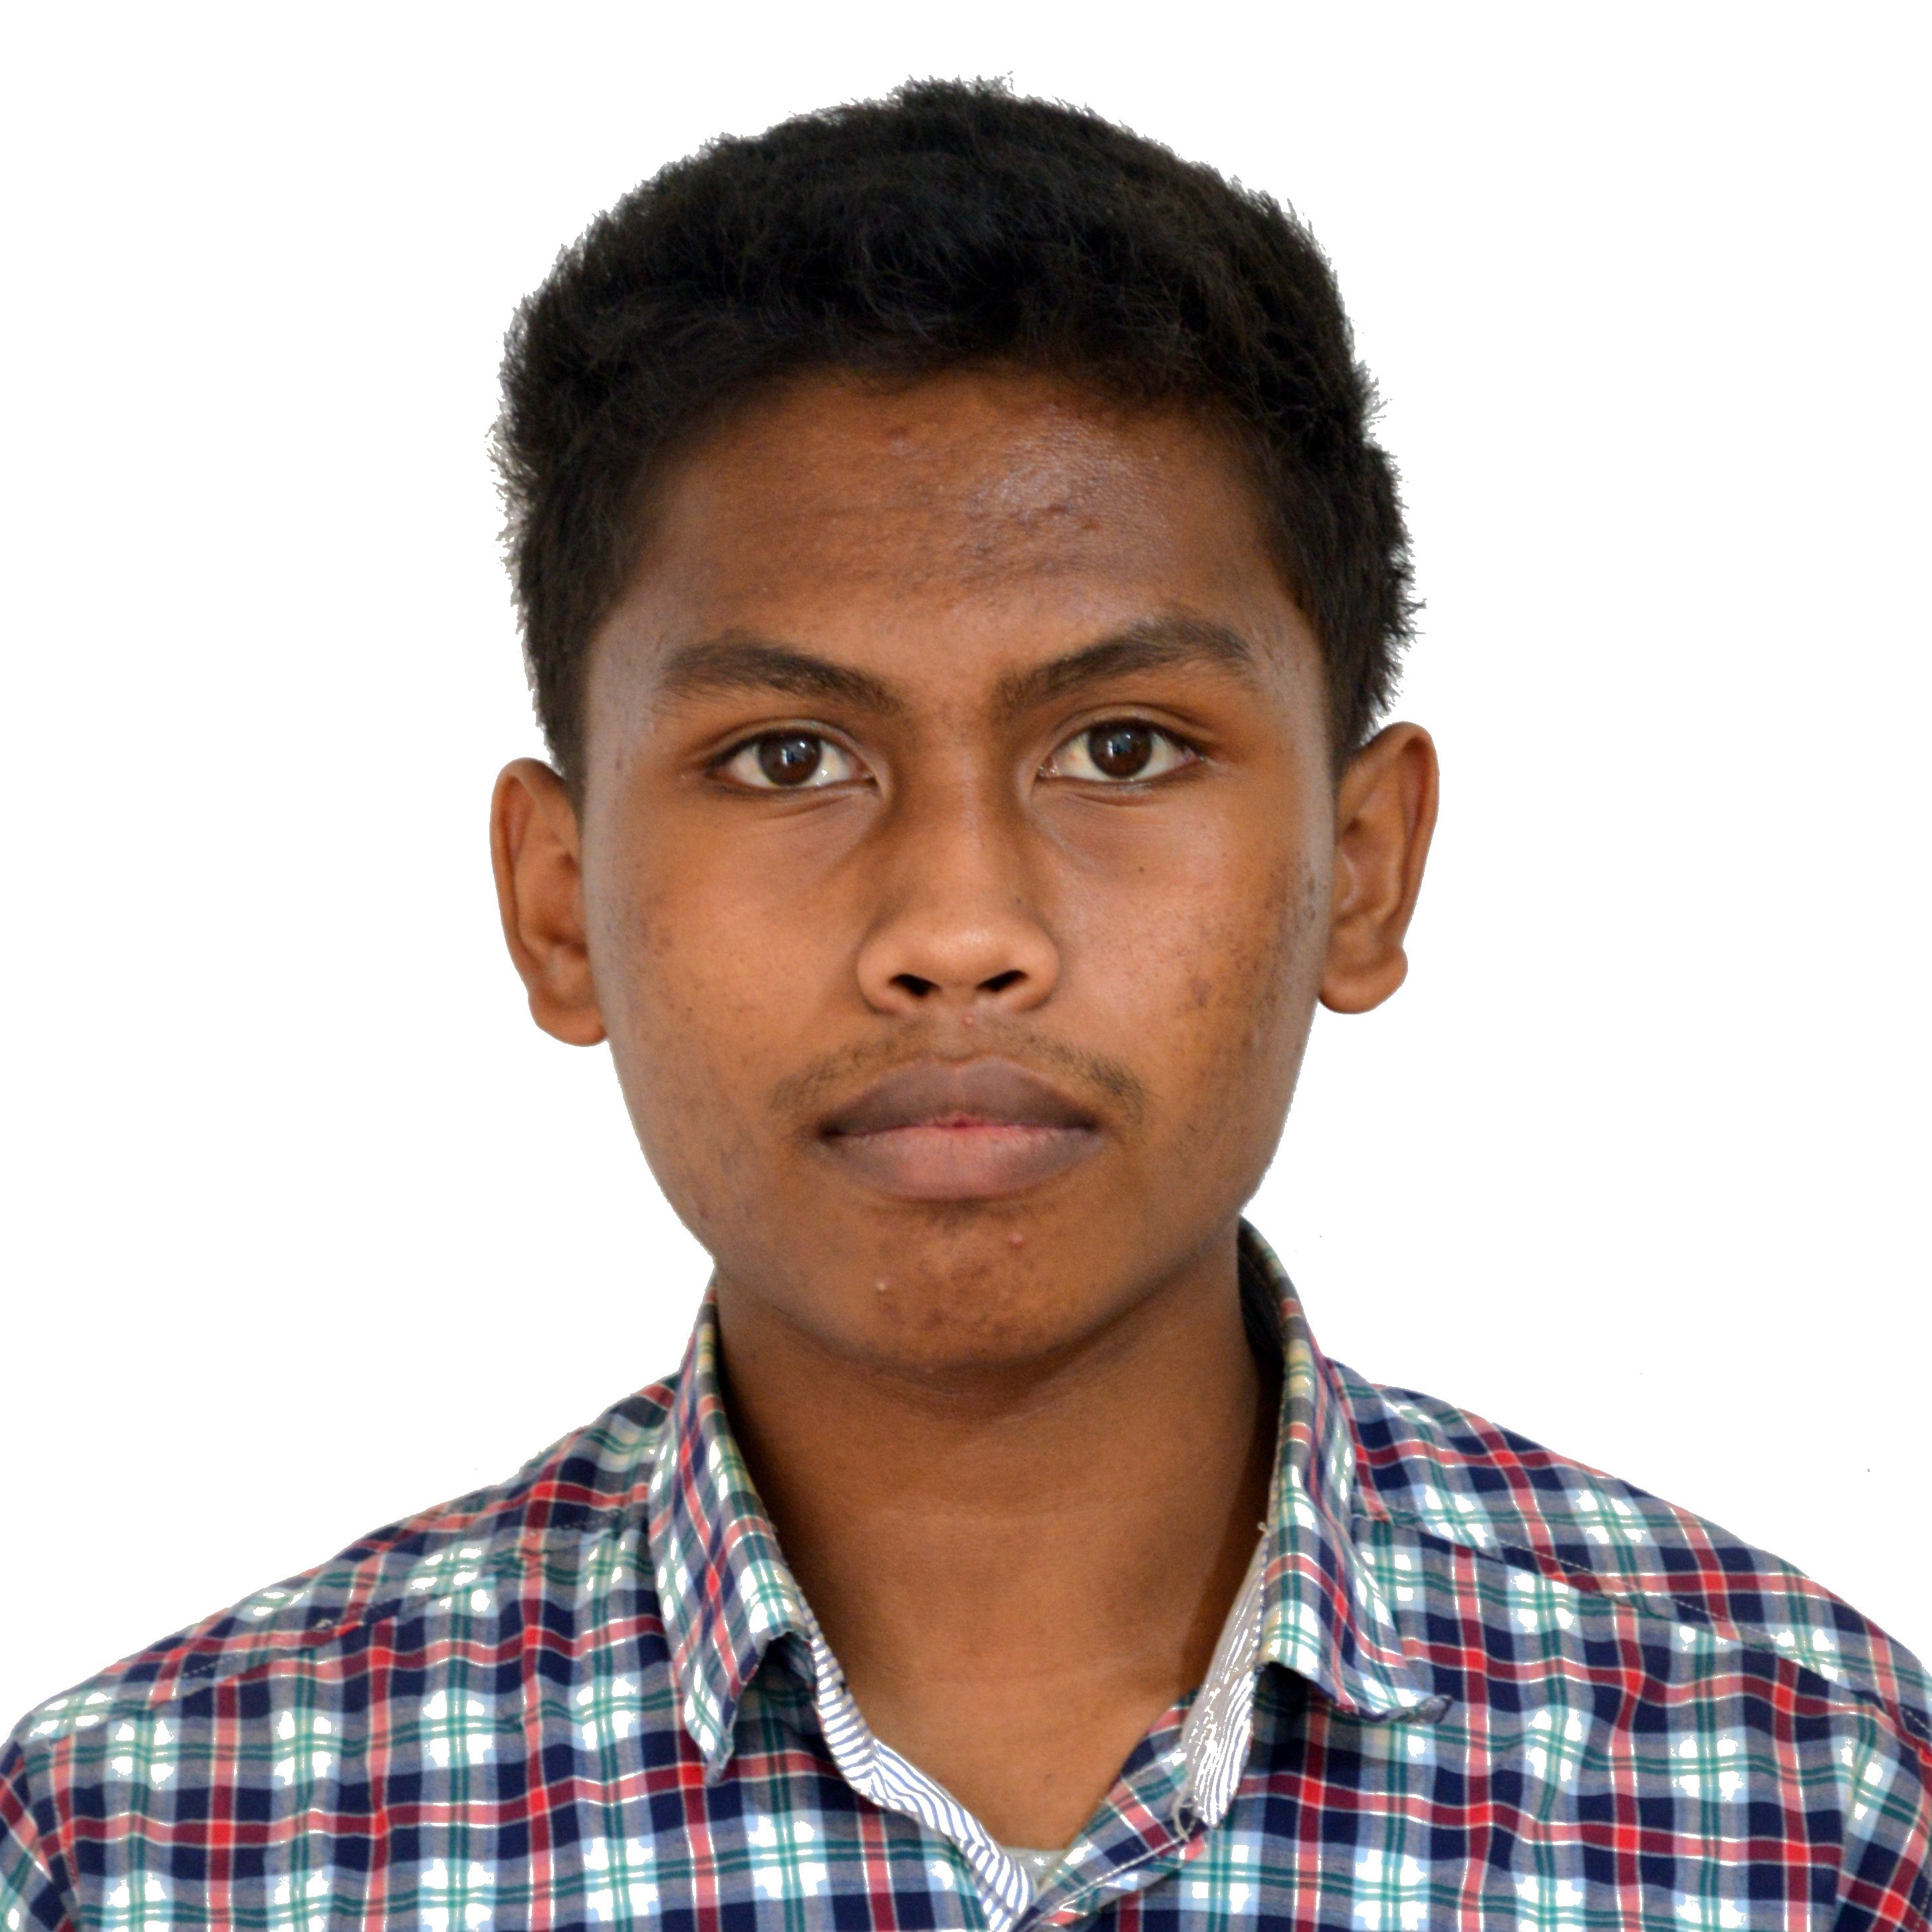
\includegraphics[width=3.5cm, height=3.5cm]{mypic.jpg}	
				\end{minipage}
			\end{center}
			\section*{FORMATIONS ET DIPLOME}
			\begin{center}
				\begin{minipage}{\textwidth}
					\textbf{2024-2025:} Deuxième année de formation en Master professionnelle à l’École Nationale d'Informatique, Université de Fianarantsoa, parcours : Informatique générale.\\[0.5cm]
					\textbf{2023-2024:} Première année de formation en Master professionnelle à l’École Nationale d'Informatique, Université de Fianarantsoa, parcours : Informatique générale.\\[0.5cm]
					\textbf{2022-2023:} Obtention du diplôme de Licence professionnelle mention Bien à l’École Nationale d'Informatique, Université de Fianarantsoa, parcours : Informatique générale.\\[0.5cm]
					\textbf{2021-2022:} Deuxième année de formation en Licence professionnelle à l’École Nationale d'Informatique, Université de Fianarantsoa, parcours : Informatique générale.\\[0.5cm]
					\textbf{2020-2021:} Première année de formation en Licence professionnelle à l’École Nationale d'Informatique, Université de Fianarantsoa, parcours : Informatique générale.\\[0.5cm]
					\textbf{2019-2020:} Obtention du diplôme de Baccalauréat série D mention assez-bien au Lycée André Résampa Antsirabe.
				\end{minipage}
			\end{center}
			\section*{STAGES ET EXPERIENCES PROFESSIONNELLES}
			\begin{center}
				\begin{minipage}{\textwidth}
       					 \textbf{11 juin 2024 au 4 novembre 2024:} Stage auprès de Nexitia technologies.
						\begin{itemize}
							\item Thème du stage: Application web Handeha voyage;
							\item Langages et outils: Java, spring boot, JavaScript, next js, Katappult, H2, UML.						
						\end{itemize}
       					 \textbf{Octobre 2023:} Projet à l’École Nationale d'Informatique.
						\begin{itemize}
							\item Thème du stage: Module de securité pour application spring boot et angular;
							\item Langages et outils: Java, spring boot, Angular, TypeScript, PostgreSQL, UML.						
						\end{itemize}       					 
					\textbf{19 octobre 2022 au 16 janvier 2023:} Stage auprès de la Paositra malagasy.
						\begin{itemize}
							\item Thème du stage: Application web pour la gestion des change;
							\item Langages et outils: Java, spring boot, Angular, TypeScript, PostgreSQL, UML.								
						\end{itemize}
					\textbf{Septembre 2022:} Projet à l’École Nationale d'Informatique.
						\begin{itemize}
							\item Thème du stage: Création d'une application mobile de gestion de cotisation de groupe;
							\item Langages et outils: Java, Android Studio.								
						\end{itemize}
					\textbf{8 mars 2021 au 7 juillet 2021:} Stage auprès du Ministère de l’Économie et de la Finance.
						\begin{itemize}
							\item Thème du stage: Application web pour la gestion des dossier du personnels de la Direction du Système d'Information;
							\item Langages et outils: Java, spring boot, Angular, TypeScript, PostgreSQL, UML.								
						\end{itemize} 
					\textbf{Avril 2021:} Projet à l’École Nationale d'Informatique.
						\begin{itemize}
							\item Thème du stage: Réalisation d’une application desktop de Gestion des heures complémentaires;
							\item Langages et outils: Php, MySQL, Ajax.								
						\end{itemize} 
					\textbf{Août 2020:} Projet à l’École Nationale d'Informatique.
						\begin{itemize}
							\item Thème du stage: Création d'une application desktop de gestion de stock;
							\item Langages et outils: C++, Qt Creator.								
						\end{itemize} 
   				\end{minipage}		
			\end{center}
			\section*{CONNAISSANCES EN INFORMATIQUE}
			\begin{center}
				\begin{minipage}{\textwidth}
					\begin{itemize}
						\item \textbf{Systèmes d'exploitation:} Microsoft Windows, Linux;
						\item \textbf{Langages de Programmation:} Java, JavaScript, TypeScript, Python , C/C++;
						\item \textbf{Développement Web:} HTML5, CSS3, Tailwind CSS, React.js, Next.js, Angular, Node.js, Express.js;
						\item \textbf{Développement Backend:} Spring Framework, Node.js, Express.js;
						\item \textbf{Compétences en bases de données:} SQL, PostgreSQL, MySQL;
						\item \textbf{Outils de Gestion de Versions:} Git, GitHub, GitLab; 	
						\item \textbf{Outils DevOps:} Docker, Kubernetes, Jenkins, Ansible;
						\item \textbf{Outils de virtualisation:} Docker, VirtualBox, VMware, Vagrant; 	
						\item \textbf{Outils de tests et Assurance Qualité:} Jest, JUnit;
						\item \textbf{Outils et Méthodologies de Conception et Gestion de Projets Logiciels:} UML, Méthodologie Agile, 2TUP, MERISE, GRASP;
						\item \textbf{Outils de Documentation et de Préparation de Contenu:} LaTeX/TeX.	
					\end{itemize}
	   			\end{minipage}		
			\end{center}
			\section*{CONNAISSANCES LINGUISTIQUE}
			\begin{center}
				\begin{minipage}{\textwidth}
					\begin{center}
						\begin{tabularx}{\textwidth}{|c|X|X|X|X|}
							\hline
							\textbf{LANGUE} & \textbf{COMPREHENSION} & \textbf{LECTURE} & \textbf{PARLE} & \textbf{ECRIT}\\
							\hline
							Anglais & Bien & Bien & Assez-bien & Bien \\
							\hline
							Français & Bien & Bien & Bien & Bien\\
							\hline
						\end{tabularx}
					\end{center}
				\end{minipage}
			\end{center}
			\section*{LOISIR ET CENTRES D'INTERET}
			\begin{center}
				\begin{minipage}{\textwidth}
					\begin{itemize}
						\item Musique;
						\item Podcast;
						\item Documentaires;
						\item Anime;
						\item Jeux video;
						\item	Lecture.
					\end{itemize}
				\end{minipage}	
			\end{center}
			\newpage
			\tableofcontents
			\newpage

			\chapter*{REMERCIEMENTS}
			\addcontentsline{toc}{chapter}{REMERCIEMENTS}	
			\begin{center}
				\begin{minipage}{\textwidth}
					\hspace{15pt} Avant toute chose, je tiens à remercier Dieu tout puissant et miséricordieux, qui m'a donné la force et la patience d'accomplir ce modeste travail.\\[0.5cm]
					Mes remerciements s’étendent également à :
					\begin{itemize}
						\item Monsieur HAJALALAINA Aimé Richard, Docteur HDR, Président de l'Université de Fianarantsoa, pour tout ce qu'il entreprend à l'Université;
						\item Monsieur MAHATODY Thomas, Docteur HDR, Directeur de l’École Nationale d'Informatique, qui nous à donné l'opportunité d'aller en stage pour ainsi permettre d’accroître nos compétences;
						\item Monsieur RANARISON Richard, Directeur Général de la Paositra Malagasy, pour son accueil et la confiance qu'il à accordée depuis mon arrivée dans l’établissement;
						\item Monsieur RATIARSON Venot, Maître de Conférences, mon encadreur pédagogique, pour ses conseils et échanges tout au long du stage;
						\item Madame RANDRIAMIHARISOA Rollande, mon encadreur professionnelle, qui m'a toujours guidée lors de la réalisation du projet;
						\item Monsieur RALAIVAO Jean Christian, Assistant d'Enseignement Supérieur et de Recherche,d’avoir accepté de présider la soutenance;
					 	\item Monsieur DIMBISOA William Germain, Docteur en Informatique, d'avoir accepté d'examiner mon présent travail;
						\item Toutes les personnels de la Paositra Malagasy, pour leurs accueils;
						\item Toutes les enseignants et les personnels de l’École Nationale d'Informatique qui se sont acharné à nous former durant l'année universitaire;
						\item Ma famille pour son soutien, que se soit moral, matériel ou financier.
					\end{itemize}
				\end{minipage}
			\end{center}
			\newpage
			\listoffigures
			\newpage
			\listoftables
			\newpage
			\chapter*{NOMENCLATURE}
			\addcontentsline{toc}{chapter}{NOMENCLATURE}	
			\newpage
			\pagenumbering{arabic}
			\setcounter{page}{1}
			\chapter*{INTRODUCTION GÉNÉRALE}
			\addcontentsline{toc}{chapter}{INTRODUCTION GÉNÉRALE}
			\begin{center}
				\begin{minipage}{\textwidth}
					\hspace{15pt} Avec sa biodiversité unique et sa richesse culturelle, Madagascar est une destination touristique de choix. Cependant, avec la demande pour des expériences de voyage personnalisées et accessibles en ligne en constante croissance, de nombreux opérateurs touristiques luttent pour obtenir la visibilité et les moyens nécessaires pour promouvoir efficacement leurs offres.\\
	
					\hspace{15pt} Malgré l'essor des plateformes de réservation en ligne, il demeure un besoin urgent d'une solution centralisée pour permettre aux opérateurs touristiques malgaches de partager leurs offres et aux voyageurs de réserver facilement leurs circuits ou séjours.\\
	
					\hspace{15pt} L'objectif de ce mémoire est de développer et de présenter "Handeha Voyage", une application web qui  facilite la mise en ligne des offres de circuits et de séjours par les opérateurs touristiques, simplifie le processus de réservation pour les utilisateurs et améliore la visibilité des opérateurs touristiques. Cette étude propose une solution novatrice qui répond directement aux défis rencontrés par les opérateurs touristiques et les voyageurs à Madagascar. En effet, l'application "Handeha Voyage" ne se contente pas de faciliter la réservation des voyages; elle redéfinit fondamentalement la manière dont les services touristiques sont présentés et consommés.\\
	
					\hspace{15pt} Ce mémoire abordera le processus de conception, de développement et de mise en œuvre de l'application "Handeha Voyage". Nous utiliserons des méthodes de conception et de modélisation adaptées, ainsi que des langages de programmation et frameworks appropriés, sans oublier un système de gestion de base de données solide. Tout cela sera orchestré selon une méthodologie de gestion de projet bien définie pour assurer une organisation optimale. Les limitations incluent le temps limité pour le développement complet de certaines fonctionnalités avancées, l'accès limité aux données et la difficulté à recueillir des retours d'expérience durant le développement.\\
	
					\hspace{15pt} Notre plan se subdivise en trois parties: dans un premier temps la présentation de l’École Nationale d'Informatique (ENI) suivie de celle de Nexitia Technology. Dans la deuxième partie, nous aborderons les analyses et la conception du projet. Enfin, la troisième partie portera sur la réalisation du projet avec les différents moyens et outils utilisés.
				\end{minipage}
			\end{center}
			\part{PRESENTATION}
			\chapter{Présentation de l’Ecole Nationale d’Informatique}
			\section{Information d’ordre générale }
				\hspace{15pt} L’Ecole Nationale d’Informatique, en abrégé ENI, est un établissement d’enseignement supérieur rattaché académiquement et administrativement à l’Université de Fianarantsoa. Le siège de l’Ecole se trouve à Tanambao-Antaninarenina à Fianarantsoa. L’adresse pour la prise de contact avec l’Ecole est la suivante : Ecole Nationale d’Informatique (ENI) Tanambao, Fianarantsoa. Le numéro de sa boîte postale est 1487 avec le code postal 301. Téléphone : 034 05 733 36 ou 032 15 204 28. Son adresse électronique est la suivante : eni@eni.mg. Il dispose également d'un site web : \textbf{www.eni.mg}
			\section{Missions et historiques}
				\hspace{15pt} L’ENI se positionne sur l’échiquier socio-éducatif malgache comme étant le plus puissant secteur de diffusion et de vulgarisation des connaissances et des technologies informatiques. 

				Cette Ecole Supérieure peut être considérée aujourd’hui comme la vitrine et la pépinière des élites informaticiennes du pays.
	
				L’Ecole s’est constituée de façon progressive au sein du Centre Universitaire Régional (CUR) de Fianarantsoa.

				De façon formelle, l’ENI était constituée et créée au sein du (CUR) par le décret N° 83- 185 du 24 Mai 1983, comme étant le seul établissement Universitaire Professionnalisé au niveau national, destiné à former des techniciens et des Ingénieurs de haut niveau, aptes à répondre aux besoins et exigences d’Informatisation des entreprises, des sociétés et des organes implantés à Madagascar.

				           \begin{center}
						\begin{minipage}{\textwidth}
								\hspace{15pt} L’ENI a pour conséquent pour mission de former des spécialistes informaticiens compétents et opérationnels de différents niveaux notamment : 
				
								\begin{itemize}
									\item En fournissant à des étudiants des connaissances de base en informatique ;
									\item En leur transmettant le savoir-faire requis, à travers la professionnalisation des formations dispensées et en essayant une meilleure adéquation des formations par rapport aux besoins évolutifs des sociétés et des entreprises ;
									\item En initiant les étudiants aux activités de recherche dans les différents domaines des Technologies de l’information et de la communication (TIC).\\
								\end{itemize}
						\end{minipage}
					\end{center}

				L’implantation de cette Ecole Supérieure de technologie de pointe dans un pays en développement et dans une Province (ou Faritany) à tissu économique et industriel faiblement développé ne l’a pourtant pas défavorisée, ni empêchée de former des spécialistes informaticiens de bon niveau, qui sont recherchés par les entreprises, les sociétés et les organismes publics et privés sur le marché de l’emploi.

				La filière de formation d’Analystes Programmeurs a été mise en place à l’Ecole en 1983, et a été gelée par la suite en 1996, tandis que la filière de formation d’ingénieurs a été ouverte à l’Ecole en 1986.
				
				Dans le cadre du Programme de renforcement en l’Enseignement Supérieur (PRESUP), la filière de formation des Techniciens Supérieurs en Maintenance des Systèmes des informatiques a été mise en place en 1986 grâce à l’appui matériel et financier de la Mission Française de coopération auprès de l’Ambassade de France à Madagascar.

				Une formation pour l’obtention de la certification CCNA et / ou NETWORK +. Appelée « CISCO Networking Academy » a été créée à l’Ecole en 2002-2003 grâce au partenariat avec CISCO SYSTEM et l’Ecole Supérieure Polytechnique d’Antananarivo (ESPA). Cependant, cette formation n’avait pas duré longtemps. Une formation de troisième cycle a été ouverte à l’Ecole a été ouverte à l’Ecole depuis l’année 2003 – 2004 grâce à la coopération académique et scientifique entre l’Université de Fianarantsoa pour le compte de l’ENI et l’Université Paul Sabatier de Toulouse (UPST).
				
				 \begin{center}
					 \begin{minipage}{\textwidth}
	
						\hspace{15pt} Cette filière avait pour objectif de former certains étudiants à la recherche dans les différents domaines de l’Informatique, et notamment pour préparer la relève des Enseignants-Chercheurs qui étaient en poste. Pendant l’année 2007-2008, la formation en vue de l’obtention du diplôme de Licence Professionnelle en Informatique a été mise en place à l’ENI avec les deux options suivantes de formation :
						
						\begin{itemize}
							\item Génie Logiciel et base de Données.
							\item Administration des Système et réseaux.\\
						\end{itemize}
					\end{minipage}

				\end{center}
				
				La mise en place à l’Ecole de ces deux options de formation devait répondre au besoin de basculement vers le système Licence – Master – Doctorat (LMD). Mais la filière de formation des Techniciens Supérieurs en Maintenance des Systèmes Informatiques a été gelée en 2009. 
En vue de surmonter les difficultés de limitation de l’effectif des étudiants accueillis à l’Ecole, notamment à cause du manque d’infrastructures, un système de « Formation Hybride » a été mise en place à partir de l’année 2010. Il s’agit en effet d’un système de formation semi présentielle et à distance avec l’utilisation de la visioconférence pour la formation à distance. Le système de formation hybride a été ainsi créé à Fianarantsoa ainsi qu’Université de Toliara.

				\section{Organigramme institutionnel}

				\hspace{15pt} Cet organigramme de l’Ecole est inspiré des dispositions du décret N° 83-185 du 23 Mai 1983.

				L’ENI est administrée par un conseil d’Ecole, et dirigée par un directeur nommé par un décret adopté en conseil des Ministres.

				Le Collège des enseignants regroupant tous les enseignants-chercheurs de l’Ecole est chargé de résoudre les problèmes liés à l’organisation pédagogique des enseignements ainsi que à l’élaboration des emplois du temps.

				\begin{center}
					\begin{minipage}{\textwidth}
						\hspace{15pt} Le Conseil Scientifique propose les orientations pédagogiques et scientifiques de l’établissement, en tenant compte notamment de l’évolution du marché de travail et de l’adéquation des formations dispensées par rapport aux besoins des entreprises. Trois départements de formation caractérisent l’organigramme :
						\begin{itemize}
							\item Le département de formation théorique à l’intérieur de l’Ecole ;
							\item Le département de formation pratique pour la coordination et la supervision des stages en entreprise et des voyages d’études ;
							\item Le département de formation doctorale pour l’organisation de la formation de 3ème cycle. La figure \ref{fig:figure 1} présente l’organigramme actuel de l’Ecole.
						\end{itemize}
					\end{minipage}
				\end{center}
				\begin{figure}[h]
					\centering
					\includegraphics[width=\textwidth]{image4.png}
					\caption{Organigramme institutionnel de l'ENI}
					\label{fig:figure 1}
				\end{figure}
				\clearpage
				
				Sur cet organigramme, l’Ecole placée sous la tutelle académique et administrative de l’Université de Fianarantsoa, et dirigée par un Directeur élu par les Enseignants – Chercheurs permanents de l’Etablissement et nommé par un décret pris en Conseil des ministres pour un mandat de 3 ans. 

				Le Conseil de l’Ecole est l’organe délibérant de l’Ecole.

				Le Collège des Enseignants propose et coordonne les programmes d’activités pédagogiques. Le Conseil scientifique coordonne les programmes de recherche à mettre en œuvre à l’Ecole. Le Secrétariat principal coordonne les activités des services administratifs (Scolarité, Comptabilité, et Intendance). Conformément aux textes en vigueur régissant les Etablissements malgaches d’Enseignement Supérieur, qui sont barrés sur le système LMD, les Départements de Formation pédagogique ont été ainsi remplacés par des Mentions et des parcours.

				Et les chefs des Départements ont été ainsi remplacés par des responsables des mentions et les responsables des parcours. Un administrateur des Réseaux et Systèmes gère le système d’information de l’Ecole et celui de l’Université.
	
				\section{Domaine de spécialisation}

				\begin{center}
					\begin{minipage}{\textwidth}
						\hspace{15pt} Les activités de formation et de recherche organisées à l’ENI portent sur les domaines suivants : 
						\begin{itemize}
							\item Génie logiciel et Base de Données ;
							\item Administration des Systèmes et Réseaux ;
							\item Informatique Générale ;
							\item Modélisation informatique et mathématique des Systèmes complexes.\\
						\end{itemize}
					\end{minipage}
				\end{center}
				D’une manière plus générale, les programmes des formations sont basés sur l’informatique de gestion et sur l’informatique des Systèmes et Réseaux. Et les modules de formation intègrent aussi bien des éléments d’Informatique fondamentale que des éléments d’Informatique appliquée. Le tableau \ref{tab:tableau 1} décrit l’organisation du système de formation pédagogique de l’Ecole.

				\begin{table}[h]
				  \centering
				  \caption{Organisation du système de formation pédagogique de l’Ecole}
				  \label{tab:tableau 1}
					  \begin{tabular}{|p{7cm}|p{7cm}|}
					    \hline
					    Formation Théorique & Formation Pratique \\
					    \hline
					    \begin{itemize}
						\item Enseignement théorique
						\item Travaux dirigés
						\item Travaux pratiques
						\item Conférences
					    \end{itemize}
					 &  
					\begin{itemize}
						\item Etude de cas
						\item Travaux de réalisation
						\item Projets/ Projets tutoriels
						\item Voyages d’Etudes
						\item Stages en entreprise
					\end{itemize}
					\\
					    \hline
					  \end{tabular}
				\end{table}
				\clearpage

				\section{Architecture des formations pédagogiques}

				\hspace{15pt} Le recrutement des étudiants à l’ENI se fait uniquement par voie de concours d’envergure nationale en première année.

				Les offres de formation organisées à l’Ecole ont été validées par la Commission Nationale d’Habilitation (CNH) auprès du Ministères de l’Enseignement Supérieur et de la Recherche Scientifique selon les dispositions de l’Arrêté N°31.174/2012-MENS en date du 05 Décembre 2012.

				\begin{center}
					\begin{minipage}{\textwidth}
						\hspace{15pt} Au sein de l’ENI, il existe une seule mention (INFORMATIQUE) et trois parcours :
						\begin{itemize}
							\item Génie logiciel et Base de Données ;
							\item Administration des Systèmes et Réseaux ; 
							\item Informatique Générale.\\
						\end{itemize}
					\end{minipage}	
				\end{center}

				L’architecture des études à trois niveaux conforment au système Licence- Master-Doctorat (LMD) permet les comparaisons et les équivalences académiques des diplômes au niveau international. 

				\begin{itemize}
					\item L = Licence (Bac + 3) = L1, L2, L3 = 6 semestres S1 à S6.

						Le diplôme de licence est obtenu en 3 années des études après Baccalauréat. Et le diplôme de Master est obtenu en 2 ans après obtenu du diplôme de LICENCE. Le MASTER PROFESSIONNEL est un diplôme destiné à la recherche emploi au terme des études.

					\item M = Master (Bac + 5) = M1, M2 = 4 semestres S7 à S10.

						Le MASTER RECHERCHE est un diplôme qui remplace l’ancien Diplôme d’Etudes Approfondies (DEA), et qui permet de s’inscrire directement dans une Ecole Doctorale.au terme des études.

					\item D = Doctorat (Bac +8).

						Le Doctorat est un diplôme qu’on peut obtenir en 3 ans après l’obtention du diplôme de MASTER RECHERCHE.\\
				\end{itemize}
				La figure \ref{fig:figure 2} présente l’architecture des études correspondant au système LMD.
				\begin{figure}[h]
					\centering
					\includegraphics[width=\textwidth]{image5.png}
					\caption{Architecture des études correspondant au système LMD}
					\label{fig:figure 2}
				\end{figure}
				\clearpage
				\noindent La licence peut avoir une vocation générale ou professionnelle.\\
				Le master peut avoir une vocation professionnelle ou de recherche.\\
				Le tableau \ref{tab:tableau 2} illustre la liste des formations existantes à l’ENI.

				\begin{table}[h]
				  \centering
				  \caption{Liste des formations existantes à l’ENI}
				  \label{tab:tableau 2}
				 \resizebox{\textwidth}{!}{
					  \begin{tabular}{|p{5cm}|p{5cm}|p{5cm}|}
						 \hline
						 & \multicolumn{2}{|c|}{FORMATION} \\
						 \hline
						 &  LICENCE PROFESSIONNELLE & MASTER \\
						 \hline
						Condition admission &
						\begin{minipage}{5cm}
						Par voie de concours\\ Formation Professionnelle: 100\\ candidats Formation généraliste: 150 candidates
						\end{minipage}
 						 &  \\
						 \hline
						Condition d’Accès & Bac de série C, D ou Technique & Être titulaire de licence professionnelle \\					
						\hline
						Durée de Formation & 3 ans & 2 ans\\
						\hline
						Diplôme délivré & Diplôme de Licence Professionnelle &
						\begin{minipage}{5cm}
						Diplôme de Master Professionnel\\Diplôme de Master Recherche
						\end{minipage}\\
						\hline
					  \end{tabular}
				}
				\end{table}

				L’accès en première année de MASTER se fait automatiquement pour les étudiants de l’Ecole qui ont obtenu le diplôme de Licence Professionnelle.

				Le Master Recherche permet à son titulaire de poursuivre directement des études en doctorat et de s’inscrire directement dans une Ecole Doctorale. 

				Les Ecoles Doctorales jouissent d’une autonomie de gestion par rapport aux Etablissements de formation universitaire.

				Il convient de signaler que par arrêté ministériel N° 21.626/2012 – MESupRES publié le 9 Août 2012 par la Commission National d’habilitation (CNH), l’Ecole Doctorale « Modélisation – Informatique » a été habilitée pour l’Université de Fianarantsoa. 

				Depuis l’année universitaire 2010-2011, l’ENI s’est mise à organiser des formations hybrides en informatique dans les différentes régions (Fianarantsoa, Toliara) en raison de l’insuffisance de la capacité d’accueil des infrastructures logistiques. En effet, le système de formation hybride semi - présentielle utilise la visioconférence pour la formation à distance. Bien qu’il n’existe pas encore au niveau international de reconnaissance écrite et formelle des diplômes délivrés par l’ENI, les étudiants diplômés de l’Ecole sont plutôt bien accueillis dans les instituts universitaires étrangères (CANADA, Suisse, France…).

				\section{Relation de l’ENI avec les organismes externes}
				
				Les stages effectués chaque année par les étudiants mettent l’Ecole en rapport permanent avec plus de 300 entreprises et organismes publics, semi-publics et privés, nationaux et internationaux.

				L’Ecole dispose ainsi d’un réseau d’entreprises, de sociétés et d’organismes publics et privés qui sont des partenaires par l’accueil en stage de ses étudiants, et éventuellement pour le recrutement après l’obtention des diplômes par ces derniers.

				Les compétences que l’Ecole cherche à développer chez ses étudiants sont l’adaptabilité, le sens de la responsabilité, du travail en équipe, le goût de l’expérimentation et l’innovation. 

				En effet, la vocation de l’ENI est de former des techniciens supérieurs de niveau LICENCE et des ingénieurs de type généraliste de niveau MASTER avec des qualités scientifiques, techniques et humaines reconnues, capables d’évoluer professionnellement dans des secteurs d’activité variés intégrant l’informatique.

				Les stages en milieu professionnel permettent de favoriser une meilleure adéquation entre les formations à l’Ecole et les besoins évolutifs du marché de l’emploi. 

				\begin{center}
					\begin{minipage}{\textwidth}
						\indent Les principaux débouchés professionnels des diplômés de l’Ecole concernent les domaines suivants :
						\begin{itemize}
							\item L’informatique de gestion d’entreprise;
							\item Les technologies de l’information et de la communication (TIC);
							\item La sécurité informatique des réseaux;
							\item L’administration des réseaux et des systèmes;
							\item Les services bancaires et financiers, notamment le Mobile Banking;
							\item Les télécommunications et la téléphonie mobile;
							\item Les Big Data;
							\item Le commerce, la vente et l’achat, le Marketing;
							\item L’ingénierie informatique appliquée;
							\item L’écologie et le développement durable.\\
						\end{itemize}
					\end{minipage}
				\end{center}

				Parmi les sociétés, entreprises et organismes partenaires de l’Ecole, on peut citer : ACCENTURE Mauritius, Air Madagascar, Ambre Associates, Airtel, Agence Universitaire de la Francophonie ( AUF) , B2B, Banque Centrale, BFG-SG, BIANCO, BLUELINE, CNaPS, Bureau National de Gestion des Risques et des Catastrophes (BNGRC), CEDII-Fianarantsoa, Data Consulting, Central Test, Centre National Antiacridien, CNRE, CHU, CNRIT, COLAS, Direction Générale des Douanes, DLC, DTS/Moov, FID, FTM, GNOSYS, GENIUS AT WORK, IBONIA, INGENOSIA, INSTAT, IOGA, JIRAMA, JOUVE, MADADEV, MAEP, MEF, MEN, MESupRES, MFB, MIC, MNINTER, Min des postes/Télécommunications et du Développement Numérique, NEOV MAD, Ny Havana, Madagascar National Parks, OMNITEC, ORANGE, OTME, PRACCESS, QMM Fort-Dauphin, SMMC, SNEDADRS Antsirabe, Sénat, Société d’Exploitation du Port de Toamasina (SEPT), SOFTWELL, Strategy Consulting, TELMA, VIVETEC, Société LAZAN’I BETSILEO, WWF … 
			
				L’organisation de stage en entreprise continue non seulement à renforcer la professionnalisation des formations dispensées, mais elle continue surtout à accroître de façon exceptionnelle les opportunités d’embauche pour les diplômés de l’Ecole.

				\section{Partenariat au niveau international}
				\begin{center}
					\begin{minipage}{\textwidth}
						\indent Entre 1996 et 1999, l’ENI avait bénéficié de l’assistance technique et financière de la Mission Française de Coopération et d’action culturelle dans le cadre du Programme de Renforcement de l’Enseignement Supérieur (PRESUP) consacré à l’Ecole a notamment porté sur :
						\begin{itemize}
							\item Une dotation en logiciels, micro-ordinateurs, équipements de laboratoire de maintenance et de matériels didactiques;
							\item La réactualisation des programmes de formation assortie du renouvellement du fonds de la bibliothèque;
							\item L’appui à la formation des formateurs;
							\item L’affectation à l’Ecole d’Assistants techniques français;\\
						\end{itemize}
					\end{minipage}
				\end{center}
				
				De 2000 à 2004, l’ENI avait fait partie des membres du bureau de la Conférence Internationale des Ecoles de formation d’Ingénieurs et Technicien d’Expression Française (CITEF). 

				Les Enseignants-Chercheurs de l’Ecole participent régulièrement aux activités organisées dans le cadre du Colloque Africain sur la Recherche en Informatique (CARI). L’ENI avait également signé un accord de coopération inter-universitaire avec l’Institut de Recherche en Mathématiques et Informatique Appliquées (IREMIA) de l’Université de la Réunion, l’Université de Rennes 1, l’INSA de Rennes, l’Institut National Polytechnique de Grenoble (INPG). 

				A partir du mois de Juillet 2001, l’ENI avait abrité le Centre de Réseau Opérationnel (Network Operating Center) du point d’accès à Internet de l’Ecole ainsi que de l’Université de Fianarantsoa. Grâce à ce projet américain qui a été financé par l’USAID Madagascar, l’ENI de l’Université de Fianarantsoa avait été dotées d’une ligne spécialisée d’accès permanent au réseau Internet.

				L’ENI avait de même noué des relations de coopération avec l’Institut de Recherche pour le Développement (IRD).

				L’objet du projet de coopération avait porté sur la modélisation environnementale du Corridor forestier de Fandriana jusqu’à Vondrozo (COFAV). Dans ce cadre, un atelier scientifique international avait été organisé à l’ENI en Septembre 2008. Cet atelier scientifique avait eu pour thème de modélisation des paysages. 

				Et dans le cadre du programme scientifique PARRUR, l’IRD avait financé depuis 2010 le projet intitulé « Forêts, Parcs et Pauvreté dans le Sud de Madagascar (FPPSM). Des étudiants en DEA et des Doctorants issus de l’ENI avaient participé à ce Programme.

				Par ailleurs, depuis toujours la même année 2010, l’ENI de Fianarantsoa avait été sélectionnée pour faire partie des organismes partenaires de l’Université de Savoie dans le cadre du projet TICEVAL relatif à la certification des compétences en TIC.

				Le projet TICEVAL avait été financé par le Fonds Francophone des Inforoutes pour la période allant de 2010 à 2012, et il avait eu pour objectif de généraliser la certification des compétences en Informatique et Internet du type C2i2e et C2imi.

				Dans le cadre du projet TICEVAL, une convention de coopération avec l’Université de Savoie avait été signée par les deux parties concernées. La mise en œuvre de la Convention de Coopération avait permis d’envoyer des étudiants de l’ENI à Chambéry pour poursuivre des études supérieures en Informatique.

				Enfin et non des moindres, l’ENI avait signé en Septembre 2009 un protocole de collaboration scientifique avec l’ESIROI – STIM de l’Université de la Réunion.

				Comme l’ENI constitue une pépinière incubatrice de technologie de pointe, d’emplois et d’entreprises, elle peut très bien servir d’instrument efficace pour renforcer la croissance économique du pays, et pour lutter contre la Pauvreté.

				De même que le statut de l’Ecole devrait permettre de renforcer la position concurrentielle de la Grande Ile sir l’orbite de la modélisation grâce au développement des nouvelles technologies.

				\section{Débouchés professionnels et diplômés}

				Le chômage des jeunes diplômés universitaires fait partie des maux qui gangrènent Madagascar. L’environnement socio-politique du pays depuis 2008 jusqu’ à ce jour a fait que le chômage des diplômés est devenu massif par rapport aux établissements de formation supérieure existants. 

				Cependant, les formations proposées par l’Ecole permettent aux diplômés d’être immédiatement opérationnels sur le marché du travail avec la connaissance d’un métier complet lié à l’informatique aux TIC. 

				L’Ecole apporte à ses étudiants un savoir-faire et un savoir-être qui les accompagnent tout au long de leur vie professionnelle. Elle a une vocation professionnalisante. 
Les diplômés en LICENCE et en MASTER issus de l’ENI peuvent faire carrière dans différents secteurs.

				L’Ecole bénéficie aujourd’hui de 34 années d’expériences pédagogiques et de reconnaissance auprès des sociétés, des entreprises et des organismes. C’est une Ecole Supérieure de référence en matière informatique.

				Par conséquent, en raison de fait que l’équipe pédagogique de l’Ecole est expérimentée, les enseignants-chercheurs et les autres formateurs de l’Ecole sont dotés d’une grande expérience dans l’enseignement et dans le milieu professionnel.

				L’Ecole est fière de collaborer de façon régulière avec un nombre croissant d’entreprises, de sociétés et d’organismes publics et privés à travers les stages des étudiants. Les formations dispensées à l’Ecole sont ainsi orientées vers le besoin et les attentes des entreprises et des sociétés. 

				L’Ecole fournit à ses étudiants de niveau LICENCE et MASTER des compétences professionnelles et métiers indispensables pour les intégrer sur le marché du travail. 
L’Ecole s’efforce de proposer à ses étudiants une double compétence à la fois technologique et managériale combinant l’informatique de gestion ainsi que l’administration des réseaux et systèmes.

				D’une manière générale, les diplômés de l’ENI n’éprouvent pas de difficultés particulières à être recrutés au terme de leurs études. Cependant, l’ENI recommande à ses diplômés de promouvoir l’entrepreneuriat en TIC et de créer des cybercafés, des SSII ou des bureaux d’études.

				Le tableau \ref{tab:tableau 3} représente les débouchés éventuels des jeunes diplômés

				\begin{table}[h]
				  \centering
				  \caption{Débouchés éventuels des jeunes diplômés}
				  \label{tab:tableau 3}
				  \resizebox{\textwidth}{!}{
				    \begin{tabular}{|p{5cm}|p{10cm}|}
				      \hline
				      LICENCE & 
				      \begin{itemize}
				        \item Analyste;
				        \item Programmeur;
				        \item Administrateur de site web/de portail web;
				        \item Assistant Informatique et internet;
				        \item Chef de projet web ou multimédia;
				        \item Développeur Informatique ou multimédia;
				        \item Intégrateur web ou web designer;
				        \item Hot liner/Hébergeur Internet;
				        \item Agent de référencement;
				        \item Technicien/Supérieur de help desk sur Informatique;
				        \item Responsable de sécurité web;
				        \item Administrateur de réseau.
				      \end{itemize} \\
				      \hline
				     MASTER & 
				      \begin{itemize}
				        \item Administrateur de réseau et système;
				        \item Architecture de système d’information;
				        \item Développeur d’applications;
				        \item Ingénieur réseau;
				        \item Webmaster / Web Designer;
				        \item Concepteur et réalisateur d’application;
				        \item Directeur du système d’informations;
				        \item Chef de projet informatique;
				        \item Responsable de sécurité informatique;
				        \item Consultant fonctionnel ou freelance.
				      \end{itemize} \\
				      \hline
				    \end{tabular}
				  }
				\end{table}
				\clearpage

				\section{Ressources humaines}
				
				\begin{itemize}
					\item Directeur de l’Ecole : Monsieur MAHATODY Thomas, Docteur HDR;
					\item Responsable de Mention : Monsieur RABETAFIKA Louis Haja, Maître de Conférences;
					\item Responsable de Parcours « Génie Logiciel et Base de Données » : Monsieur RALAIVAO Jean Christian, Assistant d’Enseignement Supérieur et de Recherche;
					\item Responsable de Parcours « Administration Systèmes et Réseaux » : Monsieur SIAKA, Assistant d’Enseignement Supérieur et de Recherche;
					\item Responsable de Parcours « Informatique Générale » : Monsieur GILANTE Gesazafy, Assistant d’Enseignement Supérieur et de Recherche;
					\item Nombre d’Enseignants permanents : 12 dont un (01) Professeur Titulaire, un (01) Professeur, un (01) Docteur HDR, cinq (05) Maîtres de Conférences et quatre (04) Assistants d’Enseignement Supérieur et de Recherche;
					\item Nombre d’Enseignants vacataires : 10;
					\item Effectif du personnel administratif : 23.
				\end{itemize}

				\chapter{Présentation de Nexitia Technologies}
				
				\chapter{Description du projet}

				\hspace{15pt} Ce chapitre présente une description détaillée du projet "Handeha Voyage", en couvrant sa nature, ses objectifs, les besoins des utilisateurs, les moyens nécessaires à sa réalisation et les résultats attendus.

				\section{Formulation}
				
				\hspace{15pt} Madagascar, avec sa biodiversité unique et sa richesse culturelle, est une destination touristique de choix. Cependant, de nombreux opérateurs touristiques rencontrent des difficultés pour obtenir la visibilité et les moyens nécessaires afin de promouvoir efficacement leurs offres. Le projet "Handeha Voyage" vise à développer une plateforme web centralisée, permettant aux opérateurs de mettre en ligne leurs offres de circuits et de séjours, et aux voyageurs de réserver facilement leurs voyages.
	
				\section{Objectifs du Projet}

				\begin{center}
					\begin{minipage}{\textwidth}
						\hspace{15pt} Les objectifs principaux de l'application "Handeha Voyage" sont les suivants :
						\begin{itemize}
							\item Amélioration de la visibilité: Augmenter la visibilité des opérateurs touristiques malgaches sur le marché numérique;
							\item Facilitation des réservations : Simplifier le processus de réservation pour les utilisateurs;
							\item Optimisation de la gestion : Fournir aux opérateurs des outils efficaces pour gérer leurs offres et leurs réservations.
						\end{itemize}
					\end{minipage}					
				\end{center}

				\section{Besoins des Utilisateurs}
				\begin{center}
					\begin{minipage}{\textwidth}
						\subsection{Besoins Fonctionnels}
						\begin{itemize}
							\item Opérateurs touristiques :
								\begin{itemize}
									\item Interface utilisateur intuitive pour mettre à jour leurs offres;
									\item Outils de gestion des réservations et des paiements;
									\item Accès à des statistiques et analyses pour optimiser leurs offres.
								\end{itemize}		
							\item Voyageurs:
								\begin{itemize}
									\item Rechercher et réserver des offres de circuits et de séjours de manière simplifiée;
									\item Consulter les avis et évaluations pour aider dans la prise de décision;
									\item Sécurité des paiements et des informations personnelles.
								\end{itemize}
						\end{itemize}
					\end{minipage}
				\end{center}

				\begin{center}
					\begin{minipage}{\textwidth}
						\subsection{Besoins Non Fonctionnels}
						\begin{itemize}
							\item \textbf{Extensibilité :}  L'application doit être extensible pour permettre l'ajout de nouvelles fonctionnalités à l'avenir;
							\item \textbf{Convivialité :} L'interface doit être simple et facile à manipuler, même pour les utilisateurs novices;
							\item \textbf{Performance :} L'application doit être rapide et capable de gérer un grand nombre de requêtes simultanées;
							\item \textbf{Sécurité :} L'application doit garantir la confidentialité et l'intégrité des données personnelles des utilisateurs.
						\end{itemize}
					\end{minipage}
				\end{center}
								
				\section{Moyens nécessaires à la réalisation du projet}
				\subsection{Moyens Humains}
				
				\hspace{15pt} Le Tableau \ref{tab:tableau 4} représente les moyens humains nécessaires à la réalisation du projet.

				\begin{table}[h]
				  \centering
				  \caption{Inventaire des moyens humains}
				  \label{tab:tableau 4}
				  \resizebox{\textwidth}{!}{
				    \begin{tabular}{|c|c|c|}
					      \hline
					      Fonction & Nombre & Rôle\\
					      \hline
					      Maître d’ouvrage & 	1  & Supervise le projet, assure les objectifs alignés avec la vision stratégique\\
					     \hline
					     Chef de projet & 1 & Coordonne toutes les activités du projet, gère les ressources et les délais\\
						\hline
 						Développeurs Web & 1 & Conçoivent, développent et maintiennent la plateforme web\\
						\hline
						Designer UX/UI & 1 & Crée l'interface utilisateur, assure une expérience utilisateur optimale\\
						\hline
				    \end{tabular}
				  }
				\end{table}
				\clearpage

				\subsection{Moyens Logiciels}

				\hspace{15pt} Le Tableau \ref{tab:tableau 5} représente les logiciels nécessaires au développement et à la mise en œuvre de "Handeha Voyage".

				\begin{table}[h]
				  \centering
				  \caption{Inventaire des moyens logiciels}
				  \label{tab:tableau 5}
				  \resizebox{\textwidth}{!}{
				    \begin{tabular}{|c|c|c|}
					      \hline
					      Désignation & Version & Utilité\\
					      \hline
					      Visual Studio Code & 1.60 & Environnement de développement\\
					     \hline
					     IntelliJ IDEA & 2021.2 & Environnement de développement intégré (IDE)\\
						\hline
 						PostgreSQL & 13.3 & Gestion de la base de données pour production\\
						\hline
						H2 & 1.4.200 & Base de données embarquée pour tests et développement\\
						\hline
						Visual Paradigm & 16.0 & Outils de modélisation et de conception\\
						\hline
						GitHub & - & Gestion des versions et collaboration\\
						\hline
						Trello & - & Gestion de projet et organisation des tâches\\
						\hline
						Slack & - & Communication et collaboration entre les membres de l'équipe\\
						\hline
						Katappult & - & Plateforme de développement low-code\\
						\hline
				    \end{tabular}
				  }
				\end{table}
				
				\subsection{Moyens matériels}
				\hspace{15pt} Le tableau \ref{tab:tableau 6} représente l’ensemble des matériels utilisés lors de la mise en œuvre de l’application :

				\begin{table}[h]
				  \centering
				  \caption{Inventaire des moyens matériels}
				  \label{tab:tableau 6}
				  \resizebox{\textwidth}{!}{
				    \begin{tabular}{|c|c|c|c|}
					      \hline
						      Désignation & Caractéristiques & Quantité & Utilité\\
					      \hline
							PC Portable & CPU: Core i7, RAM: 16 Go, SSD: 512 Go, SE: Windows 10 & 1 & Développement et tests\\
						\hline

				    \end{tabular}
				  }
				\end{table}

				\subsection{Résultats Attendus}

				\hspace{15pt} Les résultats attendus de ce projet incluent :
				
				\begin{itemize}
					\item Une augmentation de la visibilité des opérateurs touristiques malgaches;
					\item Une simplification du processus de réservation pour les utilisateurs;
					\item Une application sécurisée, fiable et facile à utiliser, répondant aux besoins des utilisateurs;
					\item Une amélioration continue basée sur les retours d'expérience des utilisateurs.
				\end{itemize}

				\subsection{Chronogramme d'activités}

				\hspace{15pt} La Figure \ref{} représente le diagramme de gant du chronogramme d'activités du projet.

				\part{ANALYSE ET CONCEPTION}
				\chapter{Analyse préalable}
				
				\hspace{15pt} Nous allons voir, dans ce chapitre, l’analyse de l’existant, les critiques de l’existant et la conception avant-projet.

				\section{Analyse de l'existant}
				
				\hspace{15pt} Pour élaborer une solution numérique efficace, il est crucial d'analyser en profondeur le système actuel. Cette analyse nous permettra de comprendre les forces et les faiblesses du système existant, afin de proposer des améliorations pertinentes.

				\subsection{Organisation actuelle}
				
				\hspace{15pt} Le secteur touristique malgache repose actuellement sur une diversité de plateformes pour la promotion des offres touristiques. Chaque opérateur utilise des outils variés, tels que des sites web individuels, des pages sur les réseaux sociaux, et des systèmes de gestion des réservations distincts. 

				En plus de ces méthodes, certains opérateurs se tournent vers des marketplaces globales comme Booking.com ou TripAdvisor pour atteindre un public international.

				 Cette approche fragmentée mène à une faible visibilité des offres touristiques locales, une complexité accrue dans la gestion des réservations, et des inefficacités opérationnelles.

				En l'absence d'une plateforme intégrée, les opérateurs doivent naviguer entre plusieurs outils, ce qui peut entraîner des redondances et des erreurs. De plus, les voyageurs rencontrent des difficultés pour comparer les offres et réserver leurs voyages de manière fluide, ce qui impacte leur expérience globale.

				\subsection{Moyens matériels et logiciels}
				\hspace{15pt} Le tableau \ref{tab:tableau 7} représente les moyens matériels et logiciels nécessaires à l'organisation actuelle :
				\begin{table}[h]
				  \centering
				  \caption{Moyens matériels et logiciels de l'organisation actuelle}
				  \label{tab:tableau 7}
				  \resizebox{\textwidth}{!}{
				    \begin{tabular}{{|p{7.5cm}|p{7.5cm}|}}
					      \hline
						     MOYENS MATÉRIELS & MOYENS LOGICIELS\\
					      \hline
							\begin{itemize}
								\item Ordinateurs
								\item Smartphones/Tablettes
								\item Serveurs
								\item Connexions Internet
								\item Imprimantes/Scanners
								\item Caméras numériques
							\end{itemize} & 
							\begin{itemize}
								\item Sites Web
								\item Réseaux Sociaux
								\item Google Sheets
								\item Logiciels de gestion interne	
								\item Plateformes de réservation
							\end{itemize}\\
						\hline

				    \end{tabular}
				  }
				\end{table}
			
				\subsection{Critique de l'existant}

				\hspace{15pt} L'analyse du système actuel de gestion des offres touristiques à Madagascar révèle plusieurs aspects positifs et défis majeurs.
				
				Le tableau \ref{tab:tableau 8} représente les points forts et les points faibles de l'organisation actuelle.
		
				\begin{table}[h]
				  \centering
				  \caption{Critique de l'organisation actuelle.}
				  \label{tab:tableau 8}
				  \resizebox{\textwidth}{!}{
				    \begin{tabular}{|p{7.5cm}|p{7.5cm}|}
					      \hline
						     POINTS FORTS & POINTS FAIBLES\\
					      \hline
							\begin{itemize}
								\item \textbf{Présence en Ligne:} Les opérateurs touristiques ont commencé à établir leur présence en ligne grâce à des sites web et des pages sur les réseaux sociaux, ce qui permet de toucher un public large et diversifié.
								\item \textbf{Accès à une Audience Internationale:} L'utilisation de plateformes comme Booking.com et TripAdvisor offre aux opérateurs une visibilité auprès d'un public international.
								\item \textbf{Communication Directe avec les Clients:} Les réseaux sociaux et les applications de messagerie comme WhatsApp et Messenger facilitent une communication rapide et directe avec les clients, ce qui est un avantage pour la gestion des demandes de renseignements et des réservations.
							\end{itemize} & 
							\begin{itemize}
								\item \textbf{Fragmentation des Plateformes:} La diversité des plateformes et des outils crée une fragmentation qui complique la gestion des réservations et des informations. : Les mises à jour des offres et des disponibilités ne sont pas synchronisées entre les différentes plateformes. Chaque opérateur utilise des systèmes différents, ce qui entraîne des redondances et des risques d'erreurs.
								\item \textbf{Coûts Élevés:} Les commissions élevées imposées par les marketplaces globales réduisent les marges bénéficiaires des opérateurs locaux, rendant difficile la compétitivité sur le marché international.
								\item \textbf{Expérience Utilisateur Fragmentée:} Les clients doivent naviguer entre plusieurs plateformes pour trouver des informations et effectuer des réservations, ce qui peut être frustrant et décourageant. L'absence d'une solution intégrée nuit à l'expérience utilisateur.
								\item \textbf{Adaptabilité Locale Insuffisante:} Les solutions actuelles, bien qu'utilisées, ne prennent pas en compte les spécificités culturelles et opérationnelles du marché malgache, limitant leur efficacité.
							\end{itemize}\\
						\hline

				    \end{tabular}
				  }
				\end{table}
				\clearpage
				\section{Conception avant projet}
				\subsection{Mise en avant du problème principal}
				
				\hspace{15pt} Les opérateurs touristiques à Madagascar rencontrent des difficultés majeures dans la gestion et la promotion de leurs offres en raison de la fragmentation des outils et des plateformes utilisés. Actuellement, chaque opérateur utilise une variété de sites web, réseaux sociaux et systèmes de gestion des réservations, ce qui entraîne des inefficacités et des incohérences.

				\subsection{Proposition de solutions}

				\hspace{15pt} Pour développer et optimiser les activités touristiques à Madagascar, les solutions suivantes ont été proposées, visant à renforcer la compétitivité et à maximiser les opportunités de croissance pour les opérateurs touristiques:

				\begin{itemize}
					\item \textbf{Solution1:} Créer une plateforme numérique centralisée dédiée à la promotion des offres touristiques et à la gestion des réservations.
					\item \textbf{Solution2:} Créer une agence de marketing numérique spécialisée dans le secteur touristique malgache.
				\end{itemize}

				Le tableau \ref{tab:tableau 9} représente les avantages et les inconvénients des deux solutions.

				\begin{table}[h]
				  \centering
				  \caption{Avantages et inconvénients des solutions proposées.}
				  \label{tab:tableau 9}
				  \resizebox{\textwidth}{!}{
				    \begin{tabular}{|p{5cm}|p{5cm}|p{5cm}|}
					      \hline
						     SOLUTION & AVANTAGES & INCONVÉNIENTS\\
					      \hline
						\textbf{Solution1:}  Créer une plateforme numérique centralisée dédiée à la promotion des offres touristiques et à la gestion des réservations. &
						\begin{itemize}
							\item Augmentation de la visibilité des offres touristiques locales.
							\item Amélioration de l'efficacité opérationnelle grâce à une gestion centralisée.
							\item Réduction des coûts de gestion et des commissions des plateformes globales.
							\item Optimisation de l'expérience utilisateur pour les clients.
						\end{itemize}
						&
						\begin{itemize}
							\item Coûts de développement et de maintenance élevés.
							\item Besoin de formation des opérateurs pour l'adoption et l'utilisation efficace de la plateforme.
							\item Risques liés à la cybersécurité et à la protection des données sensibles.
							\item Dépendance à une infrastructure technologique stable et performante.
						\end{itemize}\\						
						\hline
						\textbf{Solution2:}  Créer une agence de marketing numérique spécialisée dans le secteur touristique malgache. &
						\begin{itemize}
							\item Offre une expertise spécialisée en marketing numérique adapté au secteur touristique.
							\item Augmente la visibilité des opérateurs touristiques sur le web et les réseaux sociaux.
							\item Permet aux opérateurs de se concentrer sur leur cœur de métier tout en déléguant le marketing à des experts.
							\item Création de campagnes publicitaires ciblées pour atteindre une audience spécifique et augmenter les réservations.
						\end{itemize}
						&
						\begin{itemize}
							\item Coûts initiaux pour établir et développer l'agence.
							\item Nécessité de recruter et de former du personnel qualifié en marketing numérique.
							\item Dépendance à l'efficacité des stratégies de marketing pour générer des résultats tangibles.
							\item Risques de fluctuation des demandes et des tendances du marché.
						\end{itemize}\\						

						\hline
				    \end{tabular}
				  }
				\end{table}
				\clearpage
				\subsection{Solution retenue}

				\hspace{15pt} Pour résoudre les difficultés majeures rencontrées par les opérateurs touristiques à Madagascar dans la gestion et la promotion de leurs offres, la solution suivante a été retenue. Développer une application web centralisée, "Handeha Voyage", qui regroupe les offres touristiques de Madagascar. Cette plateforme permet aux opérateurs de mettre en ligne leurs circuits et séjours de manière cohérente et efficace.

				Cette solution simplifie le processus de réservation pour les voyageurs, améliore la visibilité des opérateurs et optimise la gestion des offres touristiques en réduisant les inefficacités dues à la fragmentation des outils actuels.

				Vu les avantages cités, la solution retenue est donc de développer "Handeha Voyage" pour centraliser les offres touristiques, améliorer la gestion et la promotion des opérateurs locaux, et simplifier le processus de réservation pour les voyageurs.

				\subsection{Méthodes utilisées}
				\subsubsection{Méthode de conception}

				\hspace{15pt} Le développement d'une application inclut inévitablement une phase de conception cruciale. Cette étape garantit que l'application atteindra les objectifs fixés tout en assurant la fiabilité des résultats et la robustesse de l'application. Elle doit respecter les contraintes de qualité, de coûts et de détails. La phase de conception facilite également le dialogue entre les concepteurs, les développeurs et les utilisateurs, servant de référence tout au long du développement et de la maintenance.

				Le tableau \ref{tab:tableau 10} recense les principaux points forts et points faibles des approches traditionnelles et les méthodes agiles.

				\begin{longtable}{|p{3cm}|p{5.5cm}|p{5.5cm}|} 
						\caption{Comparaison entre les différentes méthodes possibles pour la gestion de projet.} 
						\label{tab:tableau 10}\\ 
						\hline 
						MÉTHODES & AVANTAGES & INCONVÉNIENTS\\ 
						\hline 
						\endfirsthead 	
						\caption[]{(Suite)}\\ 
						\hline 
						MÉTHODES & AVANTAGES & INCONVÉNIENTS\\ 
						\hline 
						\endhead
						En cascade &
						\begin{itemize}
							\item \textbf{Structure claire:} Chaque phase doit être complétée avant de passer à la suivante, ce qui offre une approche structurée et séquentielle.
							\item \textbf{Documentation détaillée:} La méthode en cascade met fortement l'accent sur la documentation à chaque étape.
							\item \textbf{Facilité de gestion:} La nature séquentielle de la méthode facilite la planification et la gestion des projets.
						\end{itemize} &
						\begin{itemize}
							\item \textbf{Inflexibilité:} Difficile de revenir en arrière ou d'apporter des modifications une fois qu'une phase est terminée.
							\item \textbf{Risque accru:} Si les erreurs ne sont détectées qu'en fin de cycle, elles peuvent être coûteuses à corriger.
							\item \textbf{Temps de développement long:} Peut ralentir le processus de développement car chaque phase doit être complètement terminée avant de passer à la suivante.
						\end{itemize}\\
						\hline 
						Cycle en V &
						\begin{itemize}
							\item \textbf{Validation et vérification:} Chaque phase de développement est directement associée à une phase de test correspondante, assurant une qualité élevée.
							\item \textbf{Documentation complète:} Comme la méthode en cascade, le cycle en V met un fort accent sur la documentation.
							\item \textbf{Détection précoce des défauts:} Les tests sont planifiés dès le début, ce qui permet de détecter et de corriger les défauts plus tôt.
						\end{itemize} &
						\begin{itemize}
							\item \textbf{Rigidité:} Comme la méthode en cascade, il est difficile d'apporter des modifications en cours de route.
							\item \textbf{Coût élevé des modifications:} Les changements sont coûteux et difficiles à intégrer une fois le processus lancé.
							\item \textbf{Non adapté aux projets flexibles:} Pas idéal pour les projets où les exigences peuvent évoluer au fil du temps.
						\end{itemize}\\
						\hline 
						Méthode Agile &
						\begin{itemize}
							\item \textbf{Flexibilité:} Agile permet des ajustements rapides en fonction des retours des utilisateurs ou des changements du marché.
							\item \textbf{Livraisons fréquentes:} Les itérations courtes conduisent à des livraisons fréquentes de fonctionnalités utilisables.
							\item \textbf{Collaboration accrue:} Encourage une communication constante entre les équipes et les parties prenantes.
							\item \textbf{Réduction des risques:} Les revues régulières et les ajustements fréquents réduisent les risques de grands échecs de projet.
							\item \textbf{Satisfaction client:} Les clients voient régulièrement des progrès et peuvent influencer la direction du projet.
						\end{itemize} &
						\begin{itemize}
							\item \textbf{Manque de documentation:} La priorité sur le développement rapide peut mener à une documentation insuffisante.
							\item \textbf{Difficulté de mise à l'échelle:} Les grands projets peuvent avoir du mal à adopter Agile sans une gestion rigoureuse.
							\item \textbf{Nécessite une forte implication:} Requiert une implication constante et active des parties prenantes.
						\end{itemize}\\
						\hline 
				    \end{longtable}

				\paragraph{Choix du méthode}

				Nous avons choisi la méthodologie Agile pour le developpement de "Handeha Voyage" en raison de sa fléxibilité face aux nombreux changements du projet.
				
				Agile permet une adaptation rapide aux retours constants sur les besoins, garantissant ainsi un produit final de haute qualité.				

				\paragraph{Présentation de la méthode agile}

				\subsubsection{Méthodologie de travail}

				\hspace{15pt} Après avoir choisi la méthodologie Agile, nous devons maintenant évaluer les avantages et inconvénients des méthodes XP et SCRUM pour déterminer laquelle est la plus adaptée à notre projet.

				
				Le tableau \ref{tab:tableau 11} représente la comparaison entre XP et Scrum.


				\begin{longtable}{|p{3cm}|p{5.5cm}|p{5.5cm}|} 
						\caption{Comparaison entre XP et SCRUM.} 
						\label{tab:tableau 11}\\ 
						\hline 
						METHODE & AVANTAGES & INCONVÉNIENTS\\ 
						\hline 
						\endfirsthead 	
						\caption[]{(Suite)}\\ 
						\hline 
						METHODE & AVANTAGES & INCONVÉNIENTS\\ 
						\hline 
						\endhead
						XP (Extreme Programming) &
						\begin{itemize}
							\item Amélioration continue grâce aux feedbacks fréquents.
							\item Forte collaboration entre les membres de l'équipe.
							\item Tests fréquents pour assurer la qualité.
						\end{itemize}
						&
						\begin{itemize}
							\item Peut-être difficile à adopter pour les équipes non expérimentées.
							\item Nécessite une forte discipline et engagement.
							\item Peut être perçu comme trop rigide par certains.
						\end{itemize}\\						
						\hline
						SCRUM &
						\begin{itemize}
							\item Fléxibilité et adaptabilité aux changements.
							\item Rôles bien définis et clairs.
							\item Favorise la transparence et la communication.
						\end{itemize} &
						\begin{itemize}
							\item Peut entraîner des réunions fréquentes et chronophages.
							\item Dépendance à un Scrum Master compétent.
							\item Peut être difficile à gérer pour les grands projets.
						\end{itemize} \\
						\hline
				    \end{longtable}
				
				\paragraph{Choix du méthodologie de travail}
	
				Nous avons choisi la méthode SCRUM pour le développement de "Handeha Voyage" en raison de sa fléxibilité et de son adaptabilité aux changements fréquents.

				SCRUM favorise une communication transparente et une collaboration étroite entre les membres de l'équipe, ce qui permet de répondre rapidement aux besoins évolutifs du projet et d'assurer une livraison continue de valeur.

				\paragraph{Présentation de SCRUM}

				
				\subsubsection{Approche de développement}
				
				\hspace{15pt} Une approche de développement désigne la manière dont un projet logiciel est planifié, conçu, développé, testé et déployé. Elle inclut les méthodologies, les outils et les pratiques
utilisés pour guider le processus de développement. Les approches de développement peuvent varier en fonction des besoins du projet, des ressources disponibles et des objectifs à atteindre.

				Le développement Low Code et le développement traditionnel sont deux approches distinctes pour la création de logiciels.

				Le tableau \ref{tab:tableau 12} représente la comparaison entre Low Code et Approche Traditionnelle.

				\begin{longtable}{|p{3cm}|p{5.5cm}|p{5.5cm}|}
						\caption{Comparaison entre Low Code et Approche Traditionnelle.}
						\label{tab:tableau 12}\\ 
						\hline 
						APPROCHE & AVANTAGES & INCONVÉNIENTS\\ 
						\hline 
						\endfirsthead 	
						\caption[]{(Suite)}\\ 
						\hline 
						APPROCHE & AVANTAGES & INCONVÉNIENTS\\ 
						\hline 
						\endhead
						Low Code &
						\begin{itemize}
							\item Temps de développement plus rapide.
							\item Coût réduit.
							\item Collaboration facilitée entre les équipes métier et IT.
						\end{itemize}
						&
						\begin{itemize}
							\item Personnalisation limitée.
							\item Scalabilité parfois restreinte.
						\end{itemize}\\						
						\hline
						Approche Traditionnelle &
						\begin{itemize}
							\item Personnalisation complète.
							\item Scalabilité élevée.
							\item Contrôle total sur le code.
						\end{itemize} &
						\begin{itemize}
							\item Temps de développement plus long.
							\item Coût plus élevé.
							\item Nécessite des compétences techniques avancées.
						\end{itemize} \\
						\hline
				    \end{longtable}

				
				\paragraph{Choix de l'approche de développement}
				
				Nous avons choisi le développement Low Code pour "Handeha Voyage" en raison de sa capacité à accélérer le processus de développement et à réduire les coûts. Cette approche permet également une collaboration plus étroite entre les équipes métier et IT, ce qui est essenciel pour répondre rapidement aux besoins chnageants du projet.


				\paragraph{Présentation du Low Code}


				\subsection{Choix des outils}
				\subsubsection{Système de Gestion de Base de Données}

				\hspace{15pt} Un système de gestion de base de données (SGBD) est un logiciel qui permet à un ordinateur de stocker, récupérer, ajouter, supprimer et modifier des données, tout en assurant la sécurité, l'intégrité des données et l'uniformité des procédures administratives.


				Le tableau \ref{tab:tableau 13} représente la comparaison entre MySQL, H2 et PostgreSQL.

				\begin{longtable}{|p{3cm}|p{5.5cm}|p{5.5cm}|} 
						\caption{Comparaison entre MySQL, H2 et PostgreSQL.} 
						\label{tab:tableau 13}\\ 
						\hline 
						SGBD & AVANTAGES & INCONVÉNIENTS\\ 
						\hline 
						\endfirsthead 	
						\caption[]{(Suite)}\\ 
						\hline 
						SGBD & AVANTAGES & INCONVÉNIENTS\\ 
						\hline 
						\endhead
						MySQL. &
						\begin{itemize}
							\item \textbf{Facilité d'utilisation:} Connu pour sa simplicité et sa facilité d'utilisation, ce qui en fait un choix populaire pour les applications web.
							\item \textbf{Scalabilité:} Gère efficacement de grands ensembles de données et des sites à fort trafic.
							\item \textbf{Support communautaire:} Support communautaire étendu et large gamme d'outils d'administration.
							\item \textbf{Performance:}  Généralement meilleur pour les charges de travail intensives en écriture.
						\end{itemize}
						&
						\begin{itemize}
							\item \textbf{Fonctionnalités limitées:} Moins flexible avec les requêtes complexes et dispose de moins de fonctionnalités avancées comparé à PostgreSQL.
							\item \textbf{Problèmes de verrouillage:} Peut rencontrer des problèmes de verrouillage sous des charges de travail très concurrentielles.
							\item \textbf{Moins d'extensibilité:} Offre moins d'options pour les extensions personnalisées par rapport à PostgreSQL.
						\end{itemize}\\						
						\hline
						PostgreSQL &
						\begin{itemize}
							\item \textbf{Conformité ACID:} Assure l'intégrité des données grâce à l'atomicité, la cohérence, l'isolation et la durabilité.
							\item \textbf{Fonctionnalités avancées:} Supporte les requêtes complexes, JSON, la recherche en texte intégral et les fonctions personnalisées.
							\item \textbf{Contrôle de la concurrence:} Excellent pour gérer plusieurs transactions simultanément sans problèmes de verrouillage.
							\item \textbf{Extensibilité:} Permet l'ajout de fonctions personnalisées et d'extensions.
							\item \textbf{Intégrité des données:} Fort support des types de données, des contraintes et de la validation.
						\end{itemize} &
						\begin{itemize}
							\item \textbf{Configuration complexe:} Plus complexe à installer et à configurer par rapport à des bases de données plus simples.
							\item \textbf{Surcharge de performance:} Peut être plus lent pour des applications simples et de petite échelle en raison de sa robustesse.
							\item \textbf{Intensif en ressources:} Nécessite plus de ressources système pour fonctionner efficacement, surtout sous forte charge.
						\end{itemize} \\
						\hline
						H2&
						\begin{itemize}
							\item \textbf{Légèreté:} Utilisation minimale des ressources, ce qui le rend rapide et efficace. 	
							\item \textbf{Stockage en mémoire:} Idéal pour les environnements de test et de développement grâce à sa vitesse.
							\item \textbf{Mode intégré:} Peut être intégré aux applications Java, simplifiant ainsi la configuration.
							\item \textbf{Multi-plateforme:} Fonctionne sans problème sur plusieurs systèmes d'exploitation.
							\item \textbf{Facilité d'utilisation:} Configuration rapide et utilisation simple, parfait pour les cycles de développement rapides.
						\end{itemize}
						&
						\begin{itemize}
							\item \textbf{Scalabilité limitée:} Non conçu pour gérer des environnements à grande échelle et à haute transaction.
							\item \textbf{Non adapté à la production:} Manque de robustesse et de fonctionnalités nécessaires pour les environnements de production.
							\item \textbf{Persistance des données:} En tant que base de données en mémoire, les données sont perdues à l'arrêt de la base de données à moins d'être spécifiquement configurées pour la persistance.
						\end{itemize}\\
						\hline
				    \end{longtable}

				\paragraph{Choix du SGBD} 
				
				 PostgreSQL a été choisi pour l'environnement de production de l'application "Handeha Voyage" en raison de ses fonctionnalités avancées, de sa conformité ACID, et de sa capacité à gérer des transactions complexes et de grandes quantités de données de manière fiable. Son extensibilité et son support pour des requêtes complexes en font le candidat idéal pour une application de gestion et de promotion touristique qui nécessite une manipulation rigoureuse et sécurisée des données.

				H2 a été sélectionné pour l'environnement de développement principalement pour sa légèreté et sa rapidité. La possibilité d'exécuter H2 en mode intégré permet des cycles de développement et de test rapides et efficaces, sans les surcharges de performance et de configuration associées aux SGBD plus robustes comme PostgreSQL. Bien qu'il ne soit pas adapté pour une utilisation en production, H2 est parfait pour les phases de développement où la simplicité et la vitesse sont essentielles.				

				\paragraph{Présentation de postgreSQL}

				\paragraph{Présentation H2}

				\subsubsection{Langage de modélisation}

				\hspace{15pt} Un langage de modélisation est un langage artificiel utilisé pour exprimer des informations, des connaissances ou des systèmes dans une structure définie par un ensemble cohérent de règles. Ces règles permettent d'interpréter la signification des composants dans la structure. 

				Les langages de modelisation peuvent être graphiques ou textuels et sont utilisés dans diverses disciplines comme l'informatique, la gestion de l'information, la modélisation des processus d'affaires,le génie logiciel et l'ingénierie des systèmes.


				Le tableau \ref{tab:tableau 14} représente la comparaison entre deux langages de modélisation populaire UML et ERD.

				
				\begin{longtable}{|p{3cm}|p{5.5cm}|p{5.5cm}|} 
						\caption{Comparaison entre UML et ERD.} 
						\label{tab:tableau 14}\\ 
						\hline 
						LANGAGE & AVANTAGES & INCONVÉNIENTS\\ 
						\hline 
						\endfirsthead 	
						\caption[]{(Suite)}\\ 
						\hline 
						LANGAGE & AVANTAGES & INCONVÉNIENTS\\ 
						\hline 
						\endhead
						UML (Unified Modeling Language) &
						\begin{itemize}
							\item Standard international largement adopté.
							\item Supporte la modélisation orienté objet.
							\item Utilisé pour la conception et la documentation des systèmes logiciels complexes.
						\end{itemize}
						&
						\begin{itemize}
							\item Peut être complexe à apprendre et à maîtriser. 
							\item Nécessite des outils spécifiques pour la modélisation.
						\end{itemize}\\						
						\hline
						ERD (Entity Relashionship Diagram) &
						\begin{itemize}
							\item Simple et facile à comprendre.
							\item Idéal pour la modélisation des bases de données relationnelles.
							\item Utilisé pour représenter les entités et leurs relations.
						\end{itemize} &
						\begin{itemize}
							\item Limité à la modélisation des bases de données.
							\item Moins adapté pour la modélisation des systèmes logiciels complexes.
						\end{itemize} \\
						\hline
				    \end{longtable}

				\paragraph{Choix du langage de modélisation} 
			
				Nous avons choisi d'utiliser UML pour "Handeha Voyage" en raison de ses nombreux avantages. En tant que standard international, UML est largement adopté et supporte la modélisation orienté objet, ce qui est essentiel pour notre projet. De plus, UML permet de concevoir et de documenter des systèmes logiciels complèxes de manière claire et précise, facilitant ainsi la communication entre les membres de l'equipe et les parties prenantes.

				\paragraph{Présentation d'UML}


				\subsubsection{Langage de programmation}

				\hspace{15pt} Un langage de programmation est un système formel utilisé pour donner des instructions à un ordinateur. Il se compose de syntaxe et de sémantique permettant aux développeurs d'écrire du code que la machine peut interpréter et exécuter. Pour l'application "Handeha Voyage", les langages de programmation jouent un rôle crucial en définissant le fonctionnement de l'application, le traitement des données et l'interaction des utilisateurs avec le système.

				
				Le tableau \ref{tab:tableau 15} représente la comparaison entre quatre langages de programmation populaire Java, JavaScript, Python et C\#.
				
				\begin{longtable}{|p{3cm}|p{5.5cm}|p{5.5cm}|} 
						\caption{Comparaison entre Java, JavaScript, Python et C\#.} 
						\label{tab:tableau 15}\\ 
						\hline 
						LANGAGE & AVANTAGES & INCONVÉNIENTS\\ 
						\hline 
						\endfirsthead 	
						\caption[]{(Suite)}\\ 
						\hline 
						LANGAGE & AVANTAGES & INCONVÉNIENTS\\ 
						\hline 
						\endhead
						Java&
						\begin{itemize}
							\item Indépendant de la plateforme, grâce à la Java Virtual Machine (JVM).
							\item Performance et efficacité robustes pour les applications côté serveur.
							\item Vaste bibliothèque et cadres disponibles pour le développement.
							\item Fonctionnalités de sécurité élevées, essentielles pour gérer les données utilisateurs et les transactions financières.
						\end{itemize}
						&
						\begin{itemize}
							\item Courbe d'apprentissage plus raide comparée à certains autres langages.
							\item Code plus verbeux, ce qui peut ralentir la vitesse de développement.
						\end{itemize}\\						
						\hline
						JavaScript&
						\begin{itemize}
							\item Très polyvalent et essentiel pour le développement front-end.
							\item S'exécute nativement dans les navigateurs web, parfait pour créer des interfaces utilisateurs interactives.
							\item Large éventail de cadres qui accélèrent le développement et améliorent la fonctionnalité.
							\item Forte communauté de support et évolution continue avec de nouvelles fonctionnalités et outils.
						\end{itemize} &
						\begin{itemize}
							\item Performance historiquement plus lente pour les tâches lourdes en calcul.
							\item Peut introduire des vulnérabilités de sécurité si mal géré.
						\end{itemize} \\
						\hline
						Python &
						\begin{itemize}
							\item Facile à apprendre et à écrire, ce qui peut accélérer le développement.
							\item Ensemble riche de bibliothèques et cadres pour le développement rapide d'applications.
							\item Fort en analyse de données et apprentissage automatique, utile pour construire des systèmes de recommandation.
						\end{itemize} &
						\begin{itemize}
							\item Vitesse d'exécution plus lente comparée à Java.
							\item Moins efficace pour les applications mobiles et à grande échelle.
						\end{itemize} \\
						\hline
						C\# &
						\begin{itemize}
							\item Intégré de manière fluide avec les technologies Microsoft, parfait pour des applications Windows et cloud.
							\item Performance élevée et gestion de la mémoire efficace.
							\item Syntaxe similaire à Java, ce qui facilite l'apprentissage pour les développeurs Java.
							\item Grand écosystème avec des frameworks puissants pour le développement multi-plateforme.
						\end{itemize} &
						\begin{itemize}
							\item Principalement associé à l'écosystème Microsoft, ce qui peut limiter l'adoption sur certaines plateformes non-Microsoft.
							\item Courbe d'apprentissage pour certains frameworks spécifiques.
						\end{itemize} \\
						\hline
				    \end{longtable}

				\paragraph{Choix des langages de programmation} 

				Java a été choisi pour le back-end de l'application "Handeha Voyage" en raison de ses performances robustes, de sa sécurité et de sa scalabilité. Sa capacité à gérer des opérations complexes et de grands volumes de transactions en fait une solution idéale pour gérer les processus de réservation, les données utilisateurs et les transactions financières.

				JavaScript a été sélectionné pour le développement front-end en raison de sa capacité à créer des interfaces utilisateurs dynamiques et interactives. Avec des cadres comme React, JavaScript permet le développement d'une expérience utilisateur réactive et engageante, essentielle pour une application visant à attirer et retenir les utilisateurs.

				\paragraph{Présentation de Java} 

				\paragraph{Présentation de JavaScript} 

				\subsubsection{Framework}

				\hspace{15pt} Un framework est une structure préconçue qui fournit un ensemble de composants et d’outils pour faciliter le développement de logiciels. Utiliser un framework aide à standardiser le développement, améliore l'efficacité et réduit les erreurs en offrant des solutions éprouvées et réutilisables.
			
					\paragraph{Framework Java}

				Le tableau \ref{tab:tableau 16} représente la comparaison entre deux Framework Java populaire Spring Framework et Struts.
				
				\begin{longtable}{|p{3cm}|p{5.5cm}|p{5.5cm}|} 
						\caption{Comparaison entre Spring Framework et Struts.} 
						\label{tab:tableau 16}\\ 
						\hline 
						FRAMEWORK & AVANTAGES & INCONVÉNIENTS\\ 
						\hline 
						\endfirsthead 	
						\caption[]{(Suite)}\\ 
						\hline 
						FRAMEWORK & AVANTAGES & INCONVÉNIENTS\\ 
						\hline 
						\endhead
						Spring Framework&
						\begin{itemize}
							\item \textbf{Flexibilité:} Très flexible avec de nombreuses options de configuration, permet l'injection de dépendances et une gestion simplifiée des objets.
							\item \textbf{Modularité:} Offre une structure modulaire, permettant aux développeurs de choisir uniquement les modules dont ils ont besoin.
							\item \textbf{Écosystème Riche:} Intégration facile avec de nombreux autres frameworks et bibliothèques.
							\item \textbf{Support pour les Microservices:} Bien adapté pour les architectures de microservices.
							\item \textbf{Communauté et Documentation:} Grande communauté de développeurs et documentation abondante, facilitant la résolution des problèmes et l'apprentissage.
							\item \textbf{Spring Boot:} Simplifie encore plus le développement avec des configurations par défaut et des démarrages rapides.
						\end{itemize}
						&
						\begin{itemize}
							\item \textbf{Courbe d'Apprentissage:} Peut être complexe à apprendre pour les débutants en raison de sa richesse fonctionnelle.
							\item \textbf{Configuration:} La configuration peut devenir complexe pour des projets très personnalisés.
							\item \textbf{Abstraction:} Le niveau d'abstraction élevé peut rendre le débogage plus difficile.
						\end{itemize}\\						
						\hline
						Struts&
						\begin{itemize}
							\item \textbf{MVC (Model-View-Controller):} Suit le modèle MVC, ce qui aide à séparer la logique métier de la présentation.
							\item \textbf{Stabilité:} Étant l'un des plus anciens frameworks Java, il est très stable et mature.
							\item \textbf{Composants Réutilisables:} Offre des composants réutilisables, ce qui peut accélérer le développement.
							\item \textbf{Communauté:} A une communauté active qui maintient et améliore le framework.
						\end{itemize} &
						\begin{itemize}
							\item \textbf{Complexité:} Moins flexible et plus rigide que Spring, ce qui peut compliquer certaines personnalisations.
							\item \textbf{Configuration Manuelle:} Nécessite souvent une configuration manuelle plus détaillée par rapport à Spring Boot.
							\item \textbf{Évolutivité:} Moins bien adapté aux architectures modernes comme les microservices.
							\item \textbf{Performance:} Peut être moins performant pour les applications à grande échelle par rapport à Spring.
						\end{itemize} \\
						\hline
				    \end{longtable}

				\subparagraph{Choix du Framework Java}

				\hspace{15pt} Pour l'application "Handeha Voyage", nous avons choisi Spring Framework avec Spring Boot pour sa flexibilité, sa modularité et sa capacité à intégrer facilement d'autres technologies. Spring Boot facilite le démarrage rapide et la gestion de l'application, ce qui nous permet de développer une solution robuste, évolutive et sécurisée.

				\subparagraph{Présentation de Spring Framework et Spring Boot}

				\paragraph{Framework JavaScript}
				
				Le tableau \ref{tab:tableau 17} représente la comparaison entre deux Framework JavaScript populaire Next.js et Vue.js.


				\begin{longtable}{|p{3cm}|p{5.5cm}|p{5.5cm}|} 
						\caption{Comparaison entre Next.js et Vue.js.} 
						\label{tab:tableau 17}\\ 
						\hline 
						FRAMEWORK & AVANTAGES & INCONVÉNIENTS\\ 
						\hline 
						\endfirsthead 	
						\caption[]{(Suite)}\\ 
						\hline 
						FRAMEWORK & AVANTAGES & INCONVÉNIENTS\\ 
						\hline 
						\endhead
						Next.js&
						\begin{itemize}
							\item \textbf{Rendu Côté Serveur (SSR):} Fournit un excellent support pour le rendu côté serveur, améliorant les performances et le référencement (SEO).
							\item \textbf{Génération de Sites Statiques (SSG):} Permet de générer des sites statiques, plus rapides et sécurisés.
							\item \textbf{Système de Routage Basé sur les Fichiers:} Simplifie la création de routes avec un système basé sur les fichiers.
							\item \textbf{Performance:} Optimisé pour les performances, avec des fonctionnalités comme le découpage automatique du code et l'optimisation des images.
							\item \textbf{Flexibilité:} Peut être utilisé avec diverses technologies backend, offrant une grande flexibilité.
							\item \textbf{Communauté et Écosystème:} Grande communauté et écosystème robuste avec de nombreux plugins et extensions disponibles.
						\end{itemize}
						&
						\begin{itemize}
							\item \textbf{Courbe d'Apprentissage:} Peut être un peu difficile pour les débutants qui ne sont pas familiers avec React.
							\item \textbf{Configuration:} Nécessite une certaine configuration pour les cas d'utilisation avancés.
						\end{itemize}\\						
						\hline
						Vue.js&
						\begin{itemize}
							\item \textbf{Simplicité:} Facile à apprendre et à utiliser, avec une courbe d'apprentissage douce.
							\item \textbf{Réactivité:} Permet de créer des interfaces utilisateur réactives grâce à son système de liaison de données bidirectionnelle.
							\item \textbf{Flexibilité:} Peut être intégré progressivement dans les projets, ce qui facilite son adoption.
							\item \textbf{Modularité:} Structure modulaire, permettant de choisir les composants dont on a besoin.
							\item \textbf{Documentation:} Documentation claire et complète, ce qui facilite l'apprentissage et la mise en œuvre.
						\end{itemize} &
						\begin{itemize}
							\item \textbf{Écosystème:} Moins vaste que celui de React et Next.js, bien que suffisamment robuste pour de nombreux projets.
							\item \textbf{Performance SSR:} Moins performant pour le rendu côté serveur par rapport à Next.js.
							\item \textbf{Support Entreprise:} Moins de soutien des grandes entreprises comparé à React et Next.js.
						\end{itemize} \\
						\hline
				    \end{longtable}

				\subparagraph{Choix du Framework JavaScript}

				\hspace{15pt} Pour l'application "Handeha Voyage", nous avons choisi Next.js pour ses capacités de rendu côté serveur (SSR) et de génération de sites statiques (SSG), qui améliorent les performances et le référencement. Next.js offre également une grande flexibilité et une meilleure gestion des performances, ce qui en fait le choix idéal pour développer une application réactive et efficace.

				\subparagraph{Présentation de Next.js}

				\subsubsection{Plateforme Low-Code}

				\hspace{15pt} Une plateforme Low-Code est un environnement de développement qui permet de créer des applications avec un minimum de codage manuel. Elle utilise des interfaces graphiques et des fonctionnalités de glisser-déposer pour simplifier le processus de développement, rendant celui-ci accessible même aux utilisateurs ayant peu ou pas d'expérience en programmation. Cette approche accélère le cycle de développement et réduit la dépendance aux méthodes de programmation traditionnelles.

				\paragraph{Katappult}

				 Katappult est une plateforme low-code permettant de créer rapidement des applications web et mobiles en générant le code de l'application à partir du modèle de données. Elle offre la possibilité de modéliser visuellement des applications, de gérer facilement les données et de déployer des solutions prêtes à l’emploi, tout en permettant la personnalisation du code source.

				Le tableau \ref{tab:tableau 18} représente la comparaison entre Katappult et un autres plateforme Low-Code Budibase.

				\begin{longtable}{|p{3cm}|p{5.5cm}|p{5.5cm}|} 
						\caption{Comparaison entre Katappult et Budibase.} 
						\label{tab:tableau 18}\\ 
						\hline 
						PLATEFORME & AVANTAGES & INCONVÉNIENTS\\ 
						\hline 
						\endfirsthead 	
						\caption[]{(Suite)}\\ 
						\hline 
						PLATEFORME & AVANTAGES & INCONVÉNIENTS\\ 
						\hline 
						\endhead
						Katappult&
						\begin{itemize}
							\item \textbf{Personnalisation:} Accès au code source pour une personnalisation avancée, offrant une grande flexibilité pour les développeurs.
							\item \textbf{Vitesse de Déploiement:} Déploiement rapide avec des modules préconstruits, facilitant la mise en production rapide des applications.
							\item \textbf{Gestion des Données:} Capacités d'import/export intégrées, simplifiant la gestion des données.
							\item \textbf{Sécurité:} Fonctionnalités de sécurité robustes, incluant l'authentification intégrée et la gestion des paiements.
						\end{itemize}
						&
						\begin{itemize}
							\item \textbf{Complexité pour les Débutants:} Peut nécessiter des compétences en programmation pour des personnalisations complexes, ce qui peut être un obstacle pour les débutants.
							\item \textbf{Investissement Initial:} Nécessite un investissement initial en temps et en ressources pour la mise en place et la configuration.
						\end{itemize}\\						
						\hline
						Budibase&
						\begin{itemize}
							\item \textbf{Facilité d'Utilisation:} Interface conviviale et intuitive, idéale pour les utilisateurs non techniques.
							\item \textbf{Vitesse de Déploiement:} Déploiement rapide grâce à des composants préconstruits, permettant de gagner du temps dans le développement.
							\item \textbf{Coût Réduit:} Réduit les coûts de développement grâce à l'automatisation et aux outils intégrés.
							\item \textbf{Modularité:} Structure modulaire, permettant de choisir les composants dont on a besoin.
						\end{itemize} &
						\begin{itemize}
							\item \textbf{Personnalisation Limitée:} Moins de possibilités de personnalisation avancée par rapport à Katappult.
							\item \textbf{Sécurité de Base:} Fonctionnalités de sécurité moins robustes, nécessitant des extensions pour des besoins avancés.
							\item \textbf{Écosystème:} Écosystème plus restreint comparé à des plateformes plus établies, ce qui peut limiter les intégrations tierces.
						\end{itemize} \\
						\hline
				    \end{longtable}


				\chapter{ANALYSE CONCEPTUELLE}

				\hspace{15pt} Ce chapitre est consacré à étudier comment la méthode SCRUM est appliquée pour conduire le projet.

				\section{Désignation des rôles de l’équipe SCRUM}

				\hspace{15pt} Le projet "Handeha Voyage" adopte la méthodologie SCRUM pour garantir une gestion agile et efficace. SCRUM est un cadre de travail qui aide les équipes à structurer et à améliorer leurs processus de manière itérative et incrémentale. Il offre une base solide pour l'organisation des réunions, la gestion des artefacts, et la répartition des responsabilités, tout en laissant une flexibilité nécessaire pour s'adapter aux spécificités de chaque projet.

				Pour un projet de la complexité de "Handeha Voyage", il est essentiel de définir clairement les rôles au sein de l'équipe SCRUM. Ces rôles sont les suivants :

				\begin{itemize}
					\item \textbf{Membres de l'équipe de développement:} Ils sont responsables de la création et de la livraison des fonctionnalités du produit. L'équipe doit comprendre des experts en développement frontend et backend, ainsi que des spécialistes du domaine métier pour assurer une couverture complète des besoins du projet.
					\item \textbf{Product Owner:} Ce rôle est crucial pour la définition et la gestion des exigences du projet. Le Product Owner est responsable de la vision du produit et veille à ce que l'équipe de développement travaille sur les fonctionnalités ayant le plus de valeur pour les utilisateurs finaux.
					\item \textbf{Scrum Master:} Le Scrum Master est le facilitateur de l'équipe. Il garantit que les principes et pratiques SCRUM sont respectés et aide l'équipe à surmonter les obstacles et à améliorer continuellement ses processus.
				\end{itemize}
				
				En plus des membres traditionnels de l'équipe SCRUM, nous avons également inclus des professionnels issus des domaines du tourisme et de l'hôtellerie. Leur expertise est essentielle pour garantir que le projet "Handeha Voyage" répond aux besoins spécifiques et aux attentes des utilisateurs finaux. Ces professionnels apportent une connaissance approfondie des tendances du marché, des attentes des clients, et des meilleures pratiques dans le domaine du tourisme et de l'hôtellerie.

				\section{Etapes de l’élaboration du product backlog}

				\hspace{15pt} Le product backlog est un élément clé dans la gestion agile du projet "Handeha Voyage". Son élaboration permet de répondre à trois questions essentielles :

				\begin{itemize}
					\item Qui sont les utilisateurs ciblés ?
					\item Quelles fonctionnalités doivent être développées ?
					\item Quel sera l'ordre de livraison de ces fonctionnalités ?
				\end{itemize}

				Pour répondre à ces questions, nous suivons un processus en cinq étapes que nous allons détailler un à un.

				\subsection{Établissement de la vision du projet}

				\hspace{15pt} Cette étape consiste à définir les objectifs globaux et l'orientation stratégique du projet.

				Établir une plateforme de réservation touristique comme "Handeha Voyage" incluant : l'inscription et l'authentification sur la plateforme, la gestion des rôles et permissions des utilisateurs, la gestion des circuits et des séjours touristiques, la réservation des circuits et des séjours, le paiement des réservations, ainsi que la gestion des réservations et des paiements.

				\subsection{Liste des acteurs}

				\hspace{15pt} Il est nécessaire d'identifier et de détailler tous les intervenants et utilisateurs du système dans tous ses aspects. Pour chaque intervenant, les informations suivantes doivent être précisées : rôle, description, niveau technologique, et niveau métier.

				Le tableau \ref{tab:listeActeurs} représente la liste des acteurs du projet "Handeha Voyage".


				\begin{longtable}{|p{3cm}|p{5cm}|p{3cm}|p{3cm}|} 
						\caption{Comparaison entre Katappult et Budibase.} 
						\label{tab:listeActeurs}\\ 
						\hline 
						RÔLE & DESCRIPTION & NIVEAU TECHNOLOGIQUE & NIVEAU METIER\\ 
						\hline 
						\endfirsthead 	
						\caption[]{(Suite)}\\ 
						\hline 
						RÔLE & DESCRIPTION & NIVEAU TECHNOLOGIQUE & NIVEAU METIER\\ 
						\hline 
						\endhead
						Super Administrateur & 
	
						\begin{itemize}
							\item Gérer les utilisateurs
							\item Gérer les rôles et les permissions
							\item Gérer les régions et les thèmes 							
						\end{itemize}
						
						& Élevé&Moyenne\\
						\hline
						Administrateur Handeha Voyage & 

						\begin{itemize}
							
							\item Gérer les demandes de vendre sur la plateforme
							\item Gérer les demandes de validation des circuits et séjours
							\item Gérer les demandes de publication des circuits et séjours 
							\item Suivre les statistiques des opérations sur la plateforme

						\end{itemize}
						
						& Élevé&Élevé\\
						\hline
						Tour Opérateur & 

						\begin{itemize}
							\item Gérer les circuits et séjours
							\item Gérer les hébergements, les restaurations, les activités et les points d'intérêt des circuits et des séjours
							\item Demander la validation des circuits et séjours
							\item Demander la publication des circuits et séjours
							\item Gérer les réservations
							\item Gérer les paiements
							\item Suivre les statistiques des circuits et séjours
						\end{itemize}

						&Moyenne &Élevée\\
						\hline
						Voyageur & 

						\begin{itemize}
							\item Rechercher des voyages
							\item Réserver des voyages
							\item Payer des réservations
							\item Demander à vendre sur la plateforme							
						\end{itemize}

						&Basse &Basse\\
						\hline
				    \end{longtable}


				\subsection{Thèmes}
				
				\hspace{15pt} Les thèmes sont des regroupements de fonctionnalités similaires qui permettent d'organiser le travail de manière cohérente. 
				
				De la vision du projet et la définition de chaque acteur, on extrait facilement les thèmes suivants :
				
				\begin{itemize}
					\item Inscription et authentification sur la plateforme
					\item Géstion des utilisateurs
					\item Géstion des rôles et des permissions
					\item Géstion des régions et les thèmes 							
					\item Géstion des demandes de vendre sur la plateforme
					\item Géstion des demandes de validation des circuits et séjours
					\item Géstion des demandes de publication des circuits et séjours 											\item Suivi des statistiques des opérations sur la plateforme
					\item Géstion des circuits et séjours
					\item Géstion des hébergements, des restaurations, des activités et des points d'intérêt des circuits et des séjours
					\item Demande de validation des circuits et séjours
					\item Demande de publication des circuits et séjours
					\item Géstion des réservations
					\item Géstion des paiements
					\item Suivi des statistiques des circuits et séjours
					\item Recherche des voyages
					\item Réservation des voyages
					\item Paiement des réservations
					\item Demande de vendre sur la plateforme							

				\end{itemize}

				\subsection{Vision de la première release}

				\hspace{15pt} La première release du projet "Handeha Voyage" se concentrera sur le thème ayant la plus haute priorité, assurant ainsi une base solide pour les fonctionnalités essentielles.

				Voici l'ordre de priorité des thèmes :

				\begin{itemize}
					\item \textbf{thème 1:} Inscription et authentification sur la plateforme
					\item \textbf{thème 2:} Gestion des utilisateurs
					\item \textbf{thème 3:} Gestion des rôles et des permissions
					\item \textbf{thème 4:} Gestion des régions et les thèmes
					\item \textbf{thème 5:} Gestion des circuits et séjours
					\item \textbf{thème 6:} Recherche des voyages
					\item \textbf{thème 7:} Réservation des voyages
					\item \textbf{thème 8:} Paiement des réservations
					\item \textbf{thème 9:} Gestion des réservations
					\item \textbf{thème 10:} Gestion des paiements
					\item \textbf{thème 11:} Suivi des statistiques des opérations sur la plateforme
					\item \textbf{thème 12:} Suivi des statistiques des circuits et séjours
					\item \textbf{thème 13:} Gestion des demandes de vendre sur la plateforme
					\item \textbf{thème 14:} Gestion des demandes de validation des circuits et séjours
					\item \textbf{thème 15:} Gestion des demandes de publication des circuits et séjours
					\item \textbf{thème 16:} Gestion des hébergements, des restaurations, des activités et des points d'intérêt des circuits et des séjours
					\item \textbf{thème 17:} Demande de validation des circuits et séjours
					\item \textbf{thème 18:} Demande de publication des circuits et séjours
					\item \textbf{thème 19:} Demande de vendre sur la plateforme
				\end{itemize}

				La première release est "Inscription et authentification sur la plateforme".

				\subsection{User stories}

				\hspace{15pt} Pour comprendre les besoins et attentes des différents utilisateurs de la plateforme "Handeha Voyage", nous avons élaboré les histoires d’utilisateurs suivantes. Ces histoires permettent de capturer les fonctionnalités essentielles du point de vue des utilisateurs finaux, assurant que le développement reste centré sur l’expérience utilisateur. 

				Une User Story respecte la syntaxe suivante : En tant que …, je veux …, afin de …


				\begin{itemize}
					\item En tant que Voyageur, je veux m'inscrire et m'authentifier pour accéder à mes informations de voyage personnalisées de manière sécurisée.
					\item En tant que Tour Opérateur, je veux pouvoir m'authentifier pour gérer mes circuits, séjours, et réservations de manière sécurisée.
					\item En tant qu'Administrateur Handeha Voyage, je veux pouvoir m'authentifier pour gérer les demandes et suivre les opérations de manière sécurisée.
					\item En tant que Super Administrateur, je veux pouvoir m'authentifier pour accéder aux fonctionnalités avancées de gestion des utilisateurs et des rôles.
					\item En tant que Super Administrateur, je veux pouvoir gérer les utilisateurs sur la plateforme pour assurer que seuls les utilisateurs autorisés ont accès aux fonctionnalités appropriées
					\item En tant que Super Administrateur, je veux pouvoir gérer les rôles et les permissions afin de contrôler les accès aux différentes fonctionnalités de la plateforme.
					\item En tant que Super Administrateur, je veux pouvoir gérer les régions et les thèmes afin de permettre d'organiser les offres de voyage par région et thématique, et ainsi améliorer la navigation et la personnalisation pour les utilisateurs.
					\item En tant que Tour Opérateur, je veux pouvoir gérer les circuits et les séjours afin d'offrire des itinéraires de voyage complets pour les voyageurs.
					\item En tant que Voyageur, je veux pouvoir rechercher des voyages selon différents critères afin de trouver des options qui répondent le mieux à mes préférences et besoins.
					\item En tant que Voyageur, je veux pouvoir sélectionner et réserver un voyage afin de finaliser mes plans de voyage.
					\item En tant que Voyageur, je veux pouvoir effectuer le paiement de mes réservations en ligne de manière sécurisée afin de finaliser ma réservation.
					\item En tant que Tour Opérateur, je veux pouvoir gérer toutes les réservations de manière efficace et sécurisée afin de garantir que les demandes des voyageurs sont traitées de manière appropriée et que les informations de réservation sont à jour.
					\item En tant que Tour Opérateur, je veux pouvoir gérer les paiements de manière efficace et sécurisée afin de garantir que toutes les transactions financières liées aux réservations sont traitées correctement et en temps opportun.
					\item En tant qu'Administrateur Handeha Voyage, je veux pouvoir suivre les statistiques des opérations sur la plateforme afin de comprendre les performances, identifier les tendances, et prendre des décisions éclairées pour améliorer les services offerts.
					\item En tant que Tour Opérateur, je veux pouvoir suivre les statistiques des circuits et séjours afin de comprendre les performances de mes offres, identifier les tendances, et ajuster mes stratégies pour améliorer les services proposés aux voyageurs.
					\item En tant qu'Administrateur Handeha Voyage, je veux pouvoir gérer les demandes de vendre sur la plateforme afin de vérifier, approuver ou rejeter les demandes des vendeurs potentiels, et garantir que seuls des vendeurs qualifiés peuvent proposer leurs offres sur la plateforme.	
					\item En tant qu'Administrateur Handeha Voyage, je veux pouvoir gérer les demandes de validation des circuits et séjours afin de garantir que toutes les offres proposées respectent les normes de qualité et de sécurité avant d'être publiées sur la plateforme.
					\item En tant qu'Administrateur Handeha Voyage, je veux pouvoir gérer les demandes de publication des circuits et séjours afin de m'assurer que toutes les offres validées sont publiées de manière appropriée et en temps opportun sur la plateforme.
					\item En tant que Tour Opérateur, je veux pouvoir gérer les hébergements, les options de restauration, les activités et les points d'intérêt associés aux circuits et séjours afin de créer des offres de voyage complètes et attractives pour les voyageurs.
					\item En tant que Tour Opérateur, je veux pouvoir soumettre des demandes de validation pour mes circuits et séjours afin de garantir qu'ils respectent les normes de qualité avant d'être publiés sur la plateforme.
					\item En tant que Tour Opérateur, je veux pouvoir soumettre des demandes de publication pour mes circuits et séjours afin de les rendre disponibles aux voyageurs sur la plateforme après leur validation.
					\item En tant que Tour Opérateur, je veux pouvoir soumettre une demande pour vendre mes circuits et séjours sur la plateforme afin d'atteindre un public plus large et augmenter mes ventes.
				\end{itemize}
				
				\section{Product Backlog}

				Le product backlog est crucial car il liste toutes les fonctionnalités et améliorations nécessaires pour le projet. Il permet de prioriser les tâches, de suivre l'avancement, et de s'adapter aux changements tout en assurant la transparence et l'organisation du travail.

				Le tableau \ref{tab:productBacklog} représente le Product Backlog du projet "Handeha Voyage".

				\begin{longtable}{|p{1cm}|p{3cm}|p{2cm}|p{2cm}|p{6cm}|} 
						\caption{Product Backlog du projet "Handeha Voyage".} 
						\label{tab:productBacklog}\\ 
						\hline 
						ID ITEM& TITRE & IMPORTANCE & ESTIMATION(Jours)&DEMONSTRATION\\ 
						\hline 
						\endfirsthead 	
						\caption[]{(Suite)}\\ 
						\hline 
						ID ITEM& TITRE & IMPORTANCE & ESTIMATION(Jours)&DEMONSTRATION\\ 
						\hline 
						\endhead
						 1&S'inscrire et s'authentifier sur la plateforme&1&8&
						\begin{itemize}
							\item Créer des comptes utilisateur
							\item Vérification de l'adresse e-mail	
							\item Connexion sécurisée
							\item Déconnexion sécurisée
							\item Récupération de mot de passe
						\end{itemize}
						\\
						\hline
						 2&Gérer les utilisateurs&2&10&						
						\begin{itemize}
							\item Créer des comptes utilisateur
							\item Consulter la liste des utilisateurs
							\item Bloquer et débloquer des comptes utilisateur	
						\end{itemize}
						\\

						\hline
						 3&Gérer les rôles et les permissions&3&8&
						\begin{itemize}
							\item Créer des rôles et permissions
							 \item Modifier des rôles et permissions
							 \item Attribuer des rôles et permissions
						\end{itemize}
						\\
						\hline
						 4&Gérer les régions et les thèmes&4&5&
						\begin{itemize}
							\item Ajouter des régions et thèmes
							\item	Modifier des régions et thèmes						
							\item Supprimer des régions et thèmes
						\end{itemize}
						\\
						\hline
						 5&Gérer les circuits et séjours&5&13&
						\begin{itemize}
							\item Créer des circuits et séjours
							\item Modifier des circuits et séjours
							\item Supprimer des circuits et séjours
						\end{itemize}
						\\
						\hline
						 6&Rechercher des voyages&6&8&
						\begin{itemize}
							\item Rechercher par destination
							\item Rechercher par themes
							\item Rechercher par dates
							\item Rechercher par budget
							\item Rechercher par nombre de personne
						\end{itemize}
						\\
						\hline
						 7&Réserver des voyages&7&13&
						\begin{itemize}
							\item Sélectioner un voyage
							\item Réserver un voyage
							\item Modifier les réservations
							\item Annuler les réservations
						\end{itemize}
						\\
						\hline
						 8&Payer les réservations&8&8&
						\begin{itemize}
							\item Paiement sécurisé
							\item Historiser les paiements
						\end{itemize}
						\\
						\hline
						 9&Gérer les réservations&9&15&
						\begin{itemize}
							\item
						\end{itemize}
						\\
						\hline
						 10&Gérer les paiements&10&10&
						\begin{itemize}
							\item
						\end{itemize}
						\\
						\hline
						 11&Suivre les statistiques des opérations sur la plateforme&11&8&
						\begin{itemize}
							\item
						\end{itemize}
						\\
						\hline
						 12&Suivre les statistiques des circuits et séjours&12&7&
						\begin{itemize}
							\item
						\end{itemize}
						\\
						\hline
						 13&Gérer les demandes de vente sur la plateforme&13&6&
						\begin{itemize}
							\item
						\end{itemize}
						\\
						\hline
						 14&Gérer les demandes de validation des circuits et séjours&14&5&
						\begin{itemize}
							\item
						\end{itemize}
						\\
						\hline
						 15&Gérer les demandes de publication des circuits et séjours&15&5&
						\begin{itemize}
							\item
						\end{itemize}
						\\
						\hline
						 16&Gérer les hébergements, restaurations, activités et points d'intérêt des circuits et séjours&16&12&
						\begin{itemize}
							\item
						\end{itemize}
						\\
						\hline
						 17&Soumettre des demandes de validation des circuits et séjours&17&4&
						\begin{itemize}
							\item
						\end{itemize}
						\\
						\hline
						 18&Soumettre des demandes de publication des circuits et séjours&18&4&
						\begin{itemize}
							\item
						\end{itemize}
						\\
						\hline
						 19&Soumettre des demandes de vendre sur la plateforme&19&6&
						\begin{itemize}
							\item
						\end{itemize}
						\\
						\hline
				    \end{longtable}
	

\end{document}	